\documentclass[11pt,a4paper]{article}

\usepackage[utf8]{inputenc}
\usepackage[T1]{fontenc}
\usepackage{lmodern}
\usepackage{amsmath,amssymb,amsthm}
\usepackage{booktabs}
\usepackage{longtable}
\usepackage{enumitem}
\usepackage{hyperref}
\usepackage[margin=2.5cm]{geometry}
\usepackage{xcolor}
\usepackage{tikz}
\usetikzlibrary{arrows.meta,positioning,calc}

\definecolor{codeblue}{RGB}{30,90,156}
\definecolor{codegray}{RGB}{100,100,110}
\definecolor{codebg}{RGB}{245,247,250}

\newtheorem{theorem}{Theorem}[section]
\newtheorem{target}[theorem]{Target Theorem}
\newtheorem{boundary}[theorem]{Boundary}

\theoremstyle{definition}
\newtheorem{definition}[theorem]{Definition}

\theoremstyle{remark}
\newtheorem*{proofsketch}{Proof sketch}

\let\oldproofsketch\proofsketch
\let\endoldproofsketch\endproofsketch
\renewenvironment{proofsketch}{\oldproofsketch\sloppy}{\endoldproofsketch}

\hypersetup{
  colorlinks=true,
  linkcolor=codeblue,
  citecolor=codeblue,
  urlcolor=codeblue,
}

\title{%
  $\boldsymbol{\delta}$: The Formal Unification of Mathematics\\
  and Physics from Distinction}
\author{%
  Jonathan Washburn\\
  Recognition Physics Institute, Austin, TX, USA\\
  \texttt{jon@recognitionphysics.org}}
\date{May 2026 \quad (Draft)}

\begin{document}

\maketitle

\begin{abstract}\sloppy
We introduce $\delta$, pronounced \emph{distinction}, as a formal foundation in
which mathematics and physics factor through a single primitive act.
Mathematics is the permission theory of distinction: what distinction allows
structurally. Physics is the cost theory of distinction: what distinction costs
when comparison becomes measurable. Both readings operate on the same carrier.
The historical split between formal structure and physical law is therefore a
split in presentation, not in source.

Starting from a single primitive (the act of marking a difference), we
construct the finite $\delta$ kernel and derive the first complete number tower.
The construction proceeds: distinction acts compose into traces; trace-level
equivalence yields quotient structure; repetition length yields base-neutral
natural numbers; balanced pairs yield integers; cross-multiplied ratios yield
rationals. We prove the arithmetic laws (associativity, commutativity,
distributivity) for each level, construct internal order, an exact
signed-orbit comparator, absolute value, order transport under addition and
negation, divisibility, primality, Euclidean quotient-remainder, gcd,
coprimality, and a rational field. A Cauchy completion surface and a rational
J-cost bridge connect the construction to the existing uniqueness theorem for
the canonical reciprocal cost $J(x) = \tfrac{1}{2}(x + x^{-1}) - 1$.

Every construction carries a strength tag ($\delta$-only, $\delta$ + trace
closure, $\delta$ + choice, or classical extension) so that the proof strength
of any downstream claim is immediately auditable. All results through the
rational field are $\delta$-only: no axiom of choice, no law of excluded
middle, no axiom of infinity. The present formal corpus proves a conditional
universal-foundation certificate and isolates, as exact theorems, what is forced
versus what is a gauge at the one load-bearing joint: the forcing of the cost
function $J$. The native arbitrary-cost uniqueness blocker is resolved as a
negative. On the discrete rational carrier $J$ is \emph{not} forced: orientation
on each prime axis is an independent free choice (we construct ratio characters
that fix every other prime and flip one). On the continuous completion the
algebraic laws (reciprocal symmetry, the composition law, normalization,
continuity) force only the one-parameter \emph{family}
$F_\lambda(x) = \tfrac{1}{2}(x^\lambda + x^{-\lambda}) - 1$, which is exactly the
orbit of $J$ under the automorphism group of the positive reals under
multiplication. The calibration $\lambda^2 = 1$ selects $J$ within that family;
the value of that calibration is a multiplicative-automorphism gauge that
$\delta$ does not fix. The honest conclusion is therefore: $\delta$ forces the
cost \emph{form}, and a unit calibration fixes the gauge that selects $J$. We
package this stratification as a single machine-checked object.

Three companion papers supply the continuous carrier and geometric realization.
The functional-equation paper proves the canonical reciprocal cost on positive
ratios~\cite{Washburn2026LogicFE}. The arithmetic paper recovers number from
the Law of Logic on the continuous carrier~\cite{Washburn2026Arithmetic}. The
recognition-geometry paper connects event quotients to
comparison~\cite{Washburn2026Geometry}. The present paper sits below those
results by constructing the carrier surface from distinction itself. The
current formal state proves a conditional universal-foundation certificate:
kernel, logic, arithmetic, rational field, real-completion surface,
formal-system embedding, admissible-foundation inevitability, recognizer cost
bridge, and the resolved cost-joint stratification all compose. The cost-forcing
question is settled (as a negative): $\delta$ forces the cost form and a unit
calibration fixes the gauge that selects $J$. The only remaining open item before
an unqualified theorem is parsing historical external foundations into the
formal-system interface.
\end{abstract}

\tableofcontents

%% ===================================================================
\section{Introduction}\label{sec:intro}

\subsection{The inherited split}

This paper constructs a formal system in which mathematics and physics share
a single primitive. The primitive is an act of distinction, written $\delta$.
From it we derive the natural numbers, integers, rationals, order,
divisibility, primality, Euclidean structure, a rational field, and a cost
function whose \emph{form} is forced by symmetry and composition constraints,
with the unit calibration a gauge choice made precise in
Section~\ref{sec:cost} rather than an additional consequence of $\delta$. The
cost function is the one that Recognition Science uses to derive physical
constants from first principles (and, for the fine-structure constant, to
localize exactly which part is forced and which part is a boundary datum). Because the mathematical carrier and the physical cost function
both originate from $\delta$, the split between mathematics and physics
reduces to a split in the question asked, not a split in the subject.

The division between the two fields is old enough that it feels natural. It
is not. It is an accident of intellectual history, hardened by centuries of
separate departments, separate journals, separate notations, and separate
hiring committees. Mathematics begins with sets, types, universes, judgments,
or categorical objects. Physics begins with states, fields, particles,
manifolds, actions, Hamiltonians, and empirical constants. Both traditions
built enormous structures from their chosen primitives, and both traditions
succeeded.

But the success concealed a shared premise. Every mathematical foundation
presupposes the ability to distinguish. A set is defined by what belongs to it
and what does not. A type is defined by which terms inhabit it and which do
not. A proposition has a truth value only because true can be distinguished
from false. On the physics side, the same act appears under different names. A
measurement distinguishes one outcome from another. A field configuration has
content because it differs from other configurations. A state has identity only
because alternatives exist. The act of distinction is there in every axiom
system, every measurement, every proof. It is treated as background, too
obvious to formalize.

$\delta$ takes that background and makes it the foreground. One primitive: the
act of distinction. A finite repetition of the act is a \emph{trace}. Trace
equivalence gives sameness. Trace inequivalence gives difference. Repetition
length gives number. Balance gives sign. Cross-comparison gives ratio. Measured
comparison gives cost. Everything in the list is derived, not assumed.

\begin{figure}[ht]
\centering
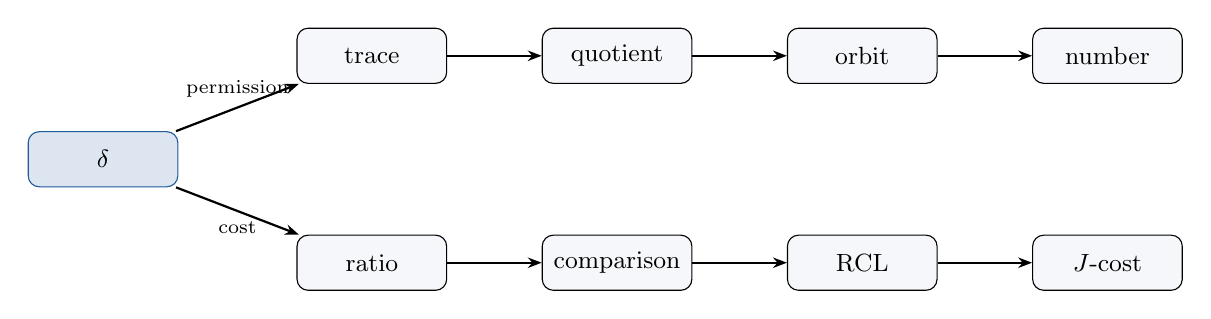
\begin{tikzpicture}[
  node distance=0.8cm and 1.6cm,
  every node/.style={font=\small},
  box/.style={draw, rounded corners=4pt, minimum width=1.9cm,
    minimum height=0.7cm, align=center, fill=codebg},
  prim/.style={box, fill=codeblue!15, draw=codeblue, font=\small\bfseries},
  arr/.style={-{Stealth[length=5pt]}, thick}
]
\node[prim] (d) {$\delta$};
\node[box, above right=0.6cm and 1.5cm of d] (trace) {trace};
\node[box, right=1.2cm of trace] (quot) {quotient};
\node[box, right=1.2cm of quot] (orbit) {orbit};
\node[box, right=1.2cm of orbit] (number) {number};

\node[box, below right=0.6cm and 1.5cm of d] (ratio) {ratio};
\node[box, right=1.2cm of ratio] (comp) {comparison};
\node[box, right=1.2cm of comp] (rcl) {RCL};
\node[box, right=1.2cm of rcl] (jcost) {$J$-cost};

\draw[arr] (d) -- (trace) node[midway, above, font=\scriptsize] {permission};
\draw[arr] (trace) -- (quot);
\draw[arr] (quot) -- (orbit);
\draw[arr] (orbit) -- (number);

\draw[arr] (d) -- (ratio) node[midway, below, font=\scriptsize] {cost};
\draw[arr] (ratio) -- (comp);
\draw[arr] (comp) -- (rcl);
\draw[arr] (rcl) -- (jcost);
\end{tikzpicture}
\caption{One act, two readings. The upper branch is permission theory
(mathematics). The lower branch is cost theory (physics). Both originate
from the same primitive $\delta$.}
\label{fig:forcing}
\end{figure}

\medskip
\noindent\textbf{Main claim.}
Mathematics and physics are formally one because both factor through
distinction. Mathematics is the permission reading of $\delta$. Physics is the
cost reading of $\delta$. Recognition Science is the program that proves,
tests, and builds the consequences of that fact.

\subsection{Contributions}

This paper makes five concrete contributions.
\begin{enumerate}[leftmargin=2em]
  \item It defines $\delta$ as a primitive foundation, not as notation for a
    prior set- or type-based carrier.
  \item It constructs a finite kernel: distinction acts, traces, trace-level
    sameness and difference, substitution, quotient recursion, and strength
    tags.
  \item It derives the first number tower through rationals as $\delta$-native
    structure: orbit length, balanced signed orbit, and cross-multiplied ratio
    orbit, with full proofs of the arithmetic laws at each level.
  \item It connects the $\delta$ carrier to the existing Recognition Science
    cost uniqueness theorem $J(x) = \tfrac{1}{2}(x + x^{-1}) - 1$.
  \item It states the current conditional universal-foundation certificate,
    resolves the cost-forcing joint as an exact stratification (form forced,
    unit a gauge), and names the one remaining external task separating that
    certificate from an unqualified theorem.
\end{enumerate}

\subsection{Status discipline}

A paper that announces a new foundation for mathematics and physics carries an
obligation that most papers do not: every claim must come with a receipt. The
temptation is to state the grand thesis and let the reader infer that the
details are worked out. We resist that. The paper separates proved content from
target content at every theorem statement, using explicit tags.

The finite kernel, trace logic, number tower, order, divisibility, Euclidean
structure, rational field surface, internal real-completion surface,
formal-system embedding theorem, admissible-foundation inevitability theorem,
recognizer cost bridge, and top-level conditional universal-foundation
certificate are proved in the present formal corpus. The cost-forcing joint is
also resolved, as an exact negative: $\delta$ forces the cost form (the gauge
orbit of $J$), a unit calibration selects $J$ within it, and the calibration
value is a gauge $\delta$ does not fix
(packaged as \texttt{PRCCostJointStratification} and
\texttt{PRCFullStratification}). The final unqualified theorem does not yet
follow: the one remaining named task is external parsing of historical
foundations into the formal-system interface. A foundation that claims to reduce
hidden assumptions must expose its own proof status, especially when the proof is
conditional.

%% ===================================================================
\section{Background}\label{sec:background}

\subsection{Existing foundations}

Four programs currently compete for the title of ``foundations of
mathematics.'' Each works. Each also leaves something on the table.

ZFC set theory, the dominant foundation since the 1920s, begins with
membership and a collection of axioms. It can encode natural numbers, integers,
rationals, reals, functions, groups, manifolds, and essentially all ordinary
mathematics. That encoding power is real. But the primitive is set membership,
and number arises only after a chain of constructions: the empty set is zero,
its singleton is one, and so on through the von Neumann ordinals. The number
three is built from three layers of set-braces. The encoding is correct, but it
carries no structural memory of what ``three'' is about. This is not a defect
in ZFC. It is a consequence of starting from a primitive (membership) that
has nothing to do with counting.

Type theory, the foundation used by modern formal proof systems, begins with types,
terms, judgments, universes, and rules. Its modern descendants are well suited
for checked mathematics. They provide the implementation environment used
in the audit behind this work. But type theory is a framework for checking arguments, not a
generator of content. It does not by itself explain why number, ratio, or cost
are forced structures rather than chosen definitions.

Category theory begins with objects, arrows, identity, and composition.
Homotopy Type Theory adds path structure and univalence. Both programs are
powerful organizers. They describe the shape of mathematical structures with
great precision. The question $\delta$ asks is different: it is not ``how
should we organize the structures we already have?''\ but ``what single
primitive act could generate those structures in the first place?''

\begin{table}[ht]
\centering
\begin{tabular}{llp{6.2cm}}
\toprule
\textbf{Program} & \textbf{Primitive surface} & \textbf{$\delta$ diagnosis} \\
\midrule
ZFC & Sets, membership &
  Good encoding; distinction is presupposed. \\
Type theory & Types, terms, judgments &
  Excellent checker; number and cost are not generated. \\
Category theory & Objects, morphisms &
  Good structural language; it describes, not generates. \\
HoTT & Types, paths, univalence &
  Good path theory; $\delta$ supplies arithmetic and cost beneath. \\
\bottomrule
\end{tabular}
\caption{Four existing foundational programs and the $\delta$ diagnosis.}
\label{tab:foundations}
\end{table}

\subsection{Recognition Science before $\delta$}

Recognition Science (RS) already had a formalized forcing chain before $\delta$
entered the picture. The functional-equation
paper~\cite{Washburn2026LogicFE} proves that on continuous positive ratios, the
reciprocal-symmetric cost satisfying the Recognition Composition Law is the
canonical reciprocal cost $J(x)=\tfrac{1}{2}(x+x^{-1})-1$. That cost is not
chosen from a menu of candidates. It is forced: the composition law itself is
the unique symmetric right-affine combiner, and then the cost on that combiner
is the unique continuous solution. The arithmetic
paper~\cite{Washburn2026Arithmetic} recovers the elementary number tower on the
same continuous carrier. The recognition-geometry
paper~\cite{Washburn2026Geometry} shows that recognizers produce event
quotients and comparison structure.

Those three papers are strong results. But they share a gap. They begin with
carriers, continuous positive ratios, event quotients, arithmetic objects, that
they take as given. A reviewer could ask: ``where did the positive ratios come
from?'' The honest answer, before $\delta$, was ``from the ambient mathematical
foundation.'' That answer is technically correct. It still undermines the
claim that RS derives physics from a single law. If the law operates on a
carrier that is imported from ZFC or type theory without comment, the
derivation has a hidden import.

$\delta$ closes that gap. Positive ratios are now ratio orbits built from
distinction. Event quotients are now trace quotients. Arithmetic carriers are
now orbit-length structures. The three companion papers remain valid, but their
starting surfaces are no longer imported. They are derived.

\subsection{Representation tax}

We introduce the term \emph{representation tax} for a specific failure mode in
foundations. A foundation pays representation tax when it encodes an object in
a way that hides the structural reason the object has its behavior. The
encoding is correct. The proof goes through. But understanding requires
reverse-engineering the structural content that the encoding stripped away.

Consider integers in ZFC. Natural numbers are sets: $0 = \{\}$,
$1 = \{\{\}\}$, $2 = \{\{\}, \{\{\}\}\}$. An integer is then an equivalence
class of pairs of naturals. The integer $-3$ is the class of all pairs $(a,b)$
with $b - a = 3$. This works. But the reason for sign, the fact that an
integer has a direction, is invisible in the encoding. You have to know the
definition of the equivalence relation to recover it. In $\delta$, an integer
is a balanced signed orbit. The positive part and the negative part are both
present. The reason for sign is in the object, not in a convention layered on
top of the object.

The same pattern appears in hard mathematics, and the cost there is higher.
A prime number in ZFC is defined as a natural number with exactly two
divisors. The definition is true. It says nothing about why primes sit where
they sit, why the gaps between primes have the distribution they have, why the
Riemann zeta function's zeros control the error term in the prime counting
function. The analytic number theorist rediscovers that structure through
150 years of sieve methods, L-functions, and analytic continuation. Some of
that work is irreducible content. But some of it is translation cost, the
price of working in a foundation where the structural reasons were removed at
the point of definition.

$\delta$ makes a testable prediction about this. If the foundation builds
primes as orbit positions with cost-structural properties from the start, some
of the translation work should disappear. How much? We do not know. That is an
empirical question about the difficulty of proofs, and we state it as such
(Section~\ref{sec:tests}).

Table~\ref{tab:reptax} gives a concrete comparison across several objects.

\begin{table}[ht]
\centering\small
\begin{tabular}{lp{4.8cm}p{4.8cm}}
\toprule
\textbf{Object} & \textbf{ZFC encoding} & \textbf{$\delta$ object} \\
\midrule
Natural number &
  Von Neumann ordinal $\{\}, \{\{\}\}, \{\{\},\{\{\}\}\}, \ldots$  &
  Orbit length of repeated distinction \\
Integer &
  Equivalence class of pairs $(a,b) \in \mathbb{N}^2$ under
  $(a,b)\sim(c,d) \Leftrightarrow a+d=b+c$ &
  Balanced signed orbit: positive and negative orbit lengths with
  balance equality $a_+ + b_- = b_+ + a_-$ \\
Rational &
  Equivalence class of pairs $(p,q) \in \mathbb{Z}\times\mathbb{Z}^*$
  under cross-multiplication &
  Ratio orbit: signed orbit over positive orbit length, with
  cross-multiplication in orbit arithmetic \\
Prime &
  $n\in\mathbb{N}$ with $|\{d : d\mid n\}|=2$ &
  Orbit position whose nontrivial factorization is forbidden
  (Thm.~\ref{thm:permission}(d)) \\
Cost &
  Not present in ZFC &
  $J(q)=\tfrac{1}{2}(q+q^{-1})-1$ on ratio orbits,
  bridged to continuous uniqueness \\
\bottomrule
\end{tabular}
\caption{Representation tax: ZFC encodes correctly but hides structural
reasons. $\delta$ represents so the reason is present in the object.}
\label{tab:reptax}
\end{table}

\subsection{Related work}

Spencer-Brown's \emph{Laws of Form}~\cite{SpencerBrown1969} is the closest
precursor. It also begins with a single primitive, the mark (or cross), and
derives a calculus from it. The key difference: Laws of Form derives Boolean
algebra. It does not derive arithmetic, and it does not produce a cost
function. $\delta$ derives both.

Conway's surreal numbers~\cite{Conway1976} generate all ordered fields from a
single recursive construction (left set, right set). This is a powerful program
with a similarly minimal starting point. The pathway is different: Conway
starts with games, not acts; and surreal numbers do not carry cost. $\delta$
generates numbers by orbit length, sign by balance, and cost by measured
comparison. The two programs are distinct pathways from a single-primitive
ambition.

Lawvere's categorical foundations~\cite{Lawvere1964} provide structural
descriptions of mathematical objects. Category theory organizes generated
structure; it does not itself generate arithmetic or cost content.
Baez~\cite{Baez2006} uses categorical methods to bridge mathematics and
physics, but the bridge is organizational, not generative. $\delta$ claims
the bridge is a shared origin, not a structural analogy.

The Univalent Foundations Program~\cite{HoTT2013} adds path structure and the
univalence axiom to type theory. HoTT excels at synthetic homotopy and identity
reasoning. $\delta$ is orthogonal: it generates arithmetic and cost from a
single primitive. HoTT could serve as a metatheory for $\delta$ quotients; the
two programs are complementary.

%% ===================================================================
\section{The $\delta$ Kernel}\label{sec:kernel}

\subsection{Distinction acts and traces}

The primitive of $\delta$ is a distinction act. The empty trace is the
absence of a performed distinction; extension adds one act. A finite trace is
a finite composition of such acts.

\begin{definition}[Distinction act]\label{def:act}
A \emph{distinction act} is a single, atomic, contentless operation of marking
a difference. It carries no parameters, no payload, no internal structure. It
is pure separation: the minimal operation that takes ``undifferentiated'' to
``differentiated.'' We write $\delta$ for this act.
\end{definition}

\begin{definition}[Trace]\label{def:trace}
A \emph{trace} is a finite sequence of distinction acts, defined inductively:
\begin{enumerate}[leftmargin=2em, label=(\roman*)]
  \item The \emph{empty trace} $\varepsilon$ is a trace (zero performed
    distinctions).
  \item If $\tau$ is a trace, then $\tau \cdot \delta$ (extending $\tau$ by
    one distinction act) is a trace.
\end{enumerate}
The \emph{length} $|\tau|$ of a trace is the number of extension steps:
$|\varepsilon| = 0$ and $|\tau \cdot \delta| = |\tau| + 1$. Trace
\emph{concatenation} $\tau_1 \mathbin{\|} \tau_2$ is defined by structural
recursion: $\tau_1 \mathbin{\|} \varepsilon = \tau_1$ and
$\tau_1 \mathbin{\|} (\tau_2 \cdot \delta) = (\tau_1 \mathbin{\|} \tau_2)
\cdot \delta$.
\end{definition}

The point is minimality. The primitive is not a set, a type, a number, a
proposition, or a physical field. It is the act by which any of those can later
be distinguished. Set theory tells you what a set is. Type theory tells you
what a type is. $\delta$ tells you what distinguishing is, and from that act,
both sets and types become available as downstream constructions rather than
starting assumptions.

\begin{theorem}[Finite trace kernel]\label{thm:kernel}
Finite distinction traces support trace extension, trace-level sameness,
trace-level difference, substitution across sameness, quotient recursion, and
the consistency condition that the same trace endpoint pair cannot be certified
both same and different in the same respect.
\end{theorem}

\begin{proof}
Trace extension is immediate from the inductive definition. Concatenation
associativity follows by structural induction on the third argument:
$(\tau_1 \mathbin{\|} \tau_2) \mathbin{\|} \varepsilon
  = \tau_1 \mathbin{\|} \tau_2
  = \tau_1 \mathbin{\|} (\tau_2 \mathbin{\|} \varepsilon)$
for the base case, and
$(\tau_1 \mathbin{\|} \tau_2) \mathbin{\|} (\tau_3 \cdot \delta)
  = ((\tau_1 \mathbin{\|} \tau_2) \mathbin{\|} \tau_3) \cdot \delta
  = (\tau_1 \mathbin{\|} (\tau_2 \mathbin{\|} \tau_3)) \cdot \delta
  = \tau_1 \mathbin{\|} ((\tau_2 \mathbin{\|} \tau_3) \cdot \delta)
  = \tau_1 \mathbin{\|} (\tau_2 \mathbin{\|} (\tau_3 \cdot \delta))$
for the inductive step, using the induction hypothesis at the third equality.

Sameness and difference are defined in Definition~\ref{def:samediff} below.
Substitution is the invariance condition (Definition~\ref{def:subst}).
Quotient recursion follows from substitution: a function $f$ on representatives
descends to a well-defined function on quotient classes whenever $f$ respects
$\sim_{\mathsf{S}}$, i.e., $a \sim_{\mathsf{S}} b$ implies $f(a) = f(b)$.
Consistency is the content of the consistency axiom
(Definition~\ref{def:samediff}).
\end{proof}

\subsection{Trace-level sameness and difference}

\begin{definition}[Trace-level sameness and difference]\label{def:samediff}
Let $A$ be a set of trace endpoints. Two binary relations on $A$ are
introduced:
\begin{enumerate}[leftmargin=2em, label=(\roman*)]
  \item A \emph{sameness} relation $a \sim_{\mathsf{S}} b$ asserts that no
    distinction in the current trace separates $a$ from $b$.
  \item A \emph{difference} relation $a \mathbin{\#} b$ asserts that some
    distinction in the trace does separate them.
\end{enumerate}
The relation $\sim_{\mathsf{S}}$ is required to be an equivalence relation
(reflexive, symmetric, transitive). The consistency axiom states that for any
fixed pair $(a,b)$ and any fixed respect, $a \sim_{\mathsf{S}} b$ and
$a \mathbin{\#} b$ cannot both hold:
\[
  \forall\, a, b \in A: \quad
  a \sim_{\mathsf{S}} b \;\;\wedge\;\; a \mathbin{\#} b
  \;\implies\; \bot.
\]
\end{definition}

This distinction between $\sim_{\mathsf{S}}$ and ordinary equality is worth
pausing on. In ZFC, equality is a logical primitive: $a = b$ is true or false
by the axiom of extensionality. In type theory, equality is the identity type
$a =_A b$. In $\delta$, sameness is a certification. The relation
$a \sim_{\mathsf{S}} b$ says that the current trace cannot distinguish $a$
from $b$. This is weaker than logical equality (different traces might
distinguish what this trace cannot) and is the right primitive for a theory
built on acts of distinction. The difference relation $a \mathbin{\#} b$
is the opposite certification: some distinction in the trace does separate
them.

The quotient surface follows. Once endpoints are identified under
$\sim_{\mathsf{S}}$, any $\delta$-native predicate must respect the
identification.

\begin{definition}[Substitution]\label{def:subst}
A predicate $P$ on trace endpoints is \emph{$\delta$-native} if it respects
sameness: whenever $a \sim_{\mathsf{S}} b$ holds, $P(a)$ implies $P(b)$.
Equivalently, $P$ descends to the quotient $A / {\sim_{\mathsf{S}}}$. This is
the invariance condition that makes quotienting well-defined: if you cannot
distinguish two things, you must not have a predicate that treats them
differently.
\end{definition}

\subsection{Strength tags}

Each theorem carries a proof-strength tag. The four main tags are:

\begin{table}[ht]
\centering
\begin{tabular}{ll}
\toprule
\textbf{Tag} & \textbf{Meaning} \\
\midrule
$\delta$-only &
  Uses only the finite distinction kernel and constructive logic. \\
$\delta$ + trace-closure &
  Adds infinite trace streams or Cauchy boundary commitments. \\
$\delta$ + choice &
  Uses a choice principle to select representatives or witnesses. \\
Classical extension &
  Uses classical real analysis or an imported classical carrier. \\
\bottomrule
\end{tabular}
\caption{Strength tags for $\delta$ theorems.}
\label{tab:strength}
\end{table}

\begin{figure}[ht]
\centering
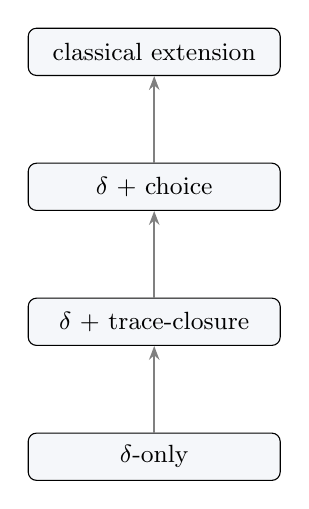
\begin{tikzpicture}[
  node distance=1.1cm,
  every node/.style={font=\small, draw, rounded corners=3pt,
    minimum width=3.2cm, minimum height=0.6cm, align=center, fill=codebg},
  arr/.style={-{Stealth[length=5pt]}, thick, gray}
]
\node (d) {$\delta$-only};
\node[above=of d] (tc) {$\delta$ + trace-closure};
\node[above=of tc] (ch) {$\delta$ + choice};
\node[above=of ch] (cl) {classical extension};
\draw[arr] (d) -- (tc);
\draw[arr] (tc) -- (ch);
\draw[arr] (ch) -- (cl);
\end{tikzpicture}
\caption{Strength-tag lattice. Each level includes the machinery of all
levels below it. The kernel and number tower live at the $\delta$-only level.
The Cauchy real surface requires trace-closure. The classical real boundary
requires classical extension.}
\label{fig:strength}
\end{figure}

The strength-tag discipline is the paper's answer to the question ``what are
your assumptions?'' In conventional mathematics, the answer is typically
something like ``ZFC plus the axiom of choice plus the law of excluded
middle,'' and this answer applies uniformly to everything in the paper. In
$\delta$, the answer is per-theorem. Each result carries its own tag, and
the tag is attached to the theorem statement. The reader can see at a glance that orbit
arithmetic is $\delta$-only (no choice, no classical logic, no infinity), that
the Cauchy real surface requires trace-closure, and that the classical real
boundary requires a full classical extension. The discipline costs the author
bookkeeping effort. It gives the reader something no other foundation
currently offers: granular proof-strength information at the theorem level.

%% ===================================================================
\section{Base-Neutral Number}\label{sec:number}

\subsection{Orbit length}

\begin{definition}[Distinction orbit ($\mathbb{N}_\delta$)]\label{def:orbit}
A \emph{distinction orbit} is an element of the inductively defined set
$\mathbb{N}_\delta$:
\begin{enumerate}[leftmargin=2em, label=(\roman*)]
  \item $0_\delta \in \mathbb{N}_\delta$ \quad (the zero orbit: no
    distinctions performed).
  \item If $n \in \mathbb{N}_\delta$, then $S_\delta(n) \in
    \mathbb{N}_\delta$ \quad (one further distinction).
\end{enumerate}
The orbit length is the number of distinction acts performed. The
\emph{display map} $\varphi : \mathbb{N}_\delta \to \mathbb{N}$ is defined by
$\varphi(0_\delta) = 0$ and $\varphi(S_\delta(n)) = \varphi(n) + 1$. This map
is the identity on the underlying count; it converts the $\delta$-native
representation into whatever numeral system is convenient.
\end{definition}

The phrase \emph{base-neutral} means that the object precedes every numeral
system. Decimal ``3'', binary ``11'', Roman ``III'', and the successor
notation $S(S(S(0)))$ are all display surfaces for the same thing: three
performed distinctions. None of those displays is the number. The number is
the orbit length:
\[
  \varepsilon \;\xrightarrow{\;\delta\;}\;
  \delta \;\xrightarrow{\;\delta\;}\;
  \delta\delta \;\xrightarrow{\;\delta\;}\;
  \delta\delta\delta \;\cdots
\]
The display map $\varphi$ converts orbit length into whatever numeral system
is convenient for a given application. This is a notational convenience, not
the source of the construction. The number existed before the display. The
tally marks on a cave wall are closer to the $\delta$ representation of number
than the Hindu-Arabic positional system, because the tally marks are direct
records of performed acts.

This matters because base-dependence is itself a form of representation tax.
When you write ``3'' in decimal, you are using a positional encoding with base
10. When you write ``11'' in binary, you are using base 2. The underlying
number is the same in both cases, and every competent mathematician knows
that. But the numeral system imports structure (positional weighting, carry
rules, zero-padding) that has nothing to do with the number. $\delta$ orbits
do not import that structure.

\subsection{Orbit arithmetic}

Addition and multiplication are defined by recursion on orbit structure,
without reference to any numeral system.

\begin{definition}[Orbit addition and multiplication]\label{def:orbitops}
Addition $\oplus$ and multiplication $\otimes$ on $\mathbb{N}_\delta$ are
defined by structural recursion on the second argument:
\begin{align}
  n \oplus 0_\delta &= n, &
  n \oplus S_\delta(m) &= S_\delta(n \oplus m); \label{eq:add} \\
  n \otimes 0_\delta &= 0_\delta, &
  n \otimes S_\delta(m) &= (n \otimes m) \oplus n. \label{eq:mul}
\end{align}
Addition is orbit concatenation: appending $m$ distinction acts after $n$.
Multiplication is repeated concatenation: $n \otimes m$ applies $n$
distinctions $m$ times. Both are $\delta$-only: no choice, no classical logic,
no axiom of infinity.
\end{definition}

\begin{theorem}[Orbit arithmetic]\label{thm:orbit}
The structure $(\mathbb{N}_\delta,\, 0_\delta,\, S_\delta,\, \oplus,\,
\otimes)$ satisfies:
\begin{enumerate}[leftmargin=2em, label=\textup{(\alph*)}]
  \item Associativity: $(a \oplus b) \oplus c = a \oplus (b \oplus c)$ and
    $(a \otimes b) \otimes c = a \otimes (b \otimes c)$.
  \item Commutativity: $a \oplus b = b \oplus a$ and
    $a \otimes b = b \otimes a$.
  \item Distributivity: $a \otimes (b \oplus c) =
    (a \otimes b) \oplus (a \otimes c)$.
  \item Identity: $a \oplus 0_\delta = a$ and
    $a \otimes S_\delta(0_\delta) = a$.
  \item Display faithfulness: $\varphi(a \oplus b) = \varphi(a) + \varphi(b)$
    and $\varphi(a \otimes b) = \varphi(a) \cdot \varphi(b)$.
\end{enumerate}
\end{theorem}

\begin{proof}
Each law follows by structural induction on $\mathbb{N}_\delta$, using the
recursive definitions~\eqref{eq:add}--\eqref{eq:mul}. We illustrate with
additive commutativity. Base case: $a \oplus 0_\delta = a = 0_\delta \oplus a$
(the second equality requires a subsidiary induction showing $0_\delta \oplus
n = n$). Inductive step: assuming $a \oplus m = m \oplus a$, we have
$a \oplus S_\delta(m) = S_\delta(a \oplus m) = S_\delta(m \oplus a)$, and a
subsidiary lemma $S_\delta(m \oplus a) = S_\delta(m) \oplus a$ completes the
step. The remaining laws follow similar inductive arguments. Display
faithfulness is a direct consequence of the recursive definitions and the
recursive definition of $\varphi$.
\end{proof}

%% ===================================================================
\section{Sign and Ratio}\label{sec:sign}

\subsection{Signed orbits}

The natural numbers have no sign. The moment you want to subtract, you need
direction. The standard construction defines integers as equivalence classes
of pairs of natural numbers, with the equivalence relation
$(a,b) \sim (c,d) \Leftrightarrow a+d = b+c$. This works. But the reason
for sign, the fact that an integer points in a direction, is invisible in
the construction. You have to know the convention (``first element is
positive, second is negative'') to extract it.

In $\delta$, sign is balance. A signed orbit is a pair of orbit lengths, one
positive and one negative. The positive part says ``this many distinctions
in the positive direction.'' The negative part says ``this many in the
negative direction.'' The signed orbit $(3, 5)$ points two steps in the
negative direction, and you can see that by looking at it.

\begin{definition}[Signed orbit]\label{def:signedorbit}
A \emph{signed orbit} is an ordered pair $(p, n) \in \mathbb{N}_\delta \times
\mathbb{N}_\delta$, where $p$ is the positive part and $n$ is the negative
part. The \emph{display} of a signed orbit is $\psi(p,n) = \varphi(p) -
\varphi(n) \in \mathbb{Z}$.

Two signed orbits $(a_+, a_-)$ and $(b_+, b_-)$ are \emph{balanced-equal},
written $(a_+, a_-) \approx (b_+, b_-)$, when
\[
  a_+ \oplus b_- \;=\; b_+ \oplus a_-
\]
in $\mathbb{N}_\delta$. This is the standard cross-addition condition, defined
entirely within orbit arithmetic. It avoids subtraction and negative numbers at
the definition level.
\end{definition}

\noindent\textbf{Example.} The integer $-1$ is represented by any pair
$(p,n)$ with $\varphi(n) = \varphi(p) + 1$: for instance,
$(0_\delta,\, S_\delta(0_\delta))$ or
$(S_\delta(0_\delta),\, S_\delta(S_\delta(0_\delta)))$. Balanced equality
identifies these: $0_\delta \oplus S_\delta(S_\delta(0_\delta))
= S_\delta(0_\delta) \oplus S_\delta(0_\delta)$.

\begin{definition}[The integers $\mathbb{Z}_\delta$]\label{def:prcint}
Define $\mathbb{Z}_\delta = (\mathbb{N}_\delta \times \mathbb{N}_\delta)
/ {\approx}$, the quotient of signed orbits by balanced equality. Operations
on $\mathbb{Z}_\delta$ are defined by lifting from representatives:
\begin{align}
  [(a_+, a_-)] + [(b_+, b_-)] &= [(a_+ \oplus b_+,\; a_- \oplus b_-)],
    \label{eq:intadd} \\
  -[(a_+, a_-)] &= [(a_-, a_+)], \label{eq:intneg} \\
  [(a_+, a_-)] \cdot [(b_+, b_-)] &= [(a_+ \otimes b_+ \oplus a_- \otimes
    b_-,\; a_+ \otimes b_- \oplus a_- \otimes b_+)]. \label{eq:intmul}
\end{align}
Each operation is well-defined on the quotient: if $(a_+, a_-) \approx
(a_+', a_-')$ and $(b_+, b_-) \approx (b_+', b_-')$, then the results are
balanced-equal.
\end{definition}

\begin{theorem}[Balanced signed orbit ring]\label{thm:int}
The balanced relation $\approx$ on signed orbits is an equivalence relation.
The quotient $\mathbb{Z}_\delta$ with the operations
\eqref{eq:intadd}--\eqref{eq:intmul} forms a commutative ring with unity
$[(S_\delta(0_\delta),\, 0_\delta)]$. The display map
$\Psi : \mathbb{Z}_\delta \to \mathbb{Z}$ defined by
$\Psi([(p,n)]) = \varphi(p) - \varphi(n)$ is a ring isomorphism.
\end{theorem}

\begin{proof}
That $\approx$ is an equivalence relation follows from the commutativity and
associativity of $\oplus$ (Theorem~\ref{thm:orbit}). Reflexivity:
$a_+ \oplus a_- = a_+ \oplus a_-$. Symmetry: if
$a_+ \oplus b_- = b_+ \oplus a_-$ then $b_+ \oplus a_- = a_+ \oplus b_-$.
Transitivity: if $a_+ \oplus b_- = b_+ \oplus a_-$ and
$b_+ \oplus c_- = c_+ \oplus b_-$, then adding these equations and canceling
$b_+$ and $b_-$ (using the cancellation law on $\mathbb{N}_\delta$, provable
by induction) yields $a_+ \oplus c_- = c_+ \oplus a_-$.

Well-definedness of addition: straightforward from the additive structure
of $\approx$. Commutativity, associativity, and distributivity follow from
the corresponding laws on $\mathbb{N}_\delta$. The display map $\Psi$ is
injective (if $\varphi(p) - \varphi(n) = \varphi(p') - \varphi(n')$ then
$(p,n) \approx (p',n')$ by the faithfulness of $\varphi$), surjective (every
integer $k$ is $\Psi([(k, 0)])$ for $k \geq 0$ or $\Psi([(0, |k|)])$ for
$k < 0$), and preserves all operations by direct computation.
\end{proof}

\begin{theorem}[Signed-orbit order, comparison, and absolute value]
\label{thm:signedorder}
Signed orbits carry an internal nonnegative predicate, strict and non-strict
order, a three-way comparison selector, and absolute value. These structures
are defined before quotienting and are compatible with balanced equality:
balanced signed orbits have the same absolute value, addition preserves and
reflects the order and comparison on either side, and negation reverses order
while preserving absolute value.
\end{theorem}

\begin{proof}
The nonnegative predicate says that a signed orbit balances with some
positive-only orbit. The computable branch selector compares the negative and
positive orbit lengths using the structural order on $\mathbb{N}_\delta$. The
absolute value is the orbit absolute difference of the two sides, not an
imported integer absolute value.

The Lean formalization proves the exact transport laws:
\[
  \operatorname{cmp}(c+a,c+b)=\operatorname{cmp}(a,b),\qquad
  \operatorname{cmp}(a+c,b+c)=\operatorname{cmp}(a,b),
\]
and
\[
  \operatorname{cmp}(-b,-a)=\operatorname{cmp}(a,b).
\]
It also proves the corresponding iff laws for $\leq$, $<$, and balanced
equality, plus $|-a|_\delta=|a|_\delta$. The display map into $\mathbb{Z}$ is
used only to verify the transport theorems; it is not used to define the
object-language order, comparator, or absolute value.
\end{proof}

\subsection{Ratio orbits}

\begin{definition}[Ratio orbit and $\mathbb{Q}_\delta$]\label{def:ratioorbit}
A \emph{ratio orbit} is a pair $(a, b)$ where $a$ is a signed orbit
(representing the numerator) and $b \in \mathbb{N}_\delta \setminus
\{0_\delta\}$ is a nonzero orbit length (the denominator). Denote the set of
ratio orbits by $\mathcal{R}$.

Two ratio orbits $(a,b)$ and $(c,d)$ are \emph{cross-equal}, written
$(a,b) \sim_\times (c,d)$, when
\[
  a \cdot \widehat{d} \;=\; c \cdot \widehat{b}
\]
in the signed-orbit multiplication of $\mathbb{Z}_\delta$, where
$\widehat{b} = [(b, 0_\delta)]$ lifts the denominator to a signed orbit with
zero negative part. Define $\mathbb{Q}_\delta = \mathcal{R} / {\sim_\times}$.
\end{definition}

\noindent\textbf{Example.} The rationals $\tfrac{2}{3}$ and $\tfrac{4}{6}$
are represented by ratio orbits with numerators $(2_\delta, 0_\delta)$ and
$(4_\delta, 0_\delta)$ and denominators $3_\delta$ and $6_\delta$
respectively. Cross equality checks
$2_\delta \otimes 6_\delta = 4_\delta \otimes 3_\delta$, i.e.,
$12_\delta = 12_\delta$ in orbit multiplication. The check uses only orbit
arithmetic; no prior notion of fraction is imported.

\begin{theorem}[Rational field from cross-multiplication]\label{thm:rat}
The cross-multiplication relation $\sim_\times$ is an equivalence relation on
$\mathcal{R}$. The quotient $\mathbb{Q}_\delta$ admits addition,
multiplication, additive inverse, and multiplicative inverse (for nonzero
elements) defined by:
\begin{align}
  [(a,b)] + [(c,d)] &= [(a \cdot \widehat{d} + c \cdot \widehat{b},\;
    b \otimes d)], \label{eq:ratadd} \\
  [(a,b)] \cdot [(c,d)] &= [(a \cdot c,\; b \otimes d)],
    \label{eq:ratmul} \\
  [(a,b)]^{-1} &= [(\epsilon_\delta(a)\widehat{b},\;
    |a|_\delta)] \quad \text{for } a \neq 0, \label{eq:ratinv}
\end{align}
where $\epsilon_\delta(a)$ is the internal signed-orbit orientation branch:
it is $+1_\delta$ when the signed-orbit nonnegative flag is true and
$-1_\delta$ otherwise. Thus the reciprocal denominator is the internal
signed-orbit absolute value, and the reciprocal numerator is selected by the
internal signed-orbit comparison, not by an imported verifier sign function.
Under these operations, $\mathbb{Q}_\delta$ is an ordered field. The display
map $\Phi : \mathbb{Q}_\delta \to \mathbb{Q}$ defined by
$\Phi([(a,b)]) = \psi(a) / \varphi(b)$ is a field isomorphism.
\end{theorem}

\begin{proof}
That $\sim_\times$ is an equivalence relation follows from the commutativity
and associativity of multiplication in $\mathbb{Z}_\delta$
(Theorem~\ref{thm:int}). Well-definedness of
\eqref{eq:ratadd}--\eqref{eq:ratinv} on the quotient follows from the
standard cross-multiplication argument: if $(a,b) \sim_\times (a',b')$ then
$a \cdot \widehat{b'} = a' \cdot \widehat{b}$, and substituting into the
operation definitions preserves cross-equality of the results. Field axioms
(commutativity, associativity, distributivity, existence of additive and
multiplicative identities and inverses) are verified by direct computation on
representatives, using the ring laws of $\mathbb{Z}_\delta$. The display map
$\Phi$ is a field isomorphism by the faithfulness of $\psi$ and $\varphi$ and
the fact that standard rational equality is also defined by
cross-multiplication.
\end{proof}

%% ===================================================================
\section{Permission Theory}\label{sec:permission}

Permission theory is the mathematical reading of $\delta$. It asks: given the
act of distinction, what structures are forced to exist before anyone assigns a
cost, makes a measurement, or does an experiment?

The answer covers most of elementary number theory. From the finite kernel alone, without
infinite trace closure, without choice, without classical logic, we get:
counting, sign, ratio, order, absolute value, divisibility, units, primality,
Euclidean division, greatest common divisors, coprimality, and a rational
field. All of it is $\delta$-only. All of it is constructive. All of it is
proved by explicit induction, quotient descent, and display-faithfulness
arguments.

This is the sense in which mathematics is ``what distinction permits.'' You do
not choose to have prime numbers. You do not define divisibility as a
convention. Once you have repeated distinction (orbits) and orbit
multiplication, divisibility is forced. Once you have divisibility, primes are
forced. The structure was always going to appear. The only question is whether
the foundation lets you see it at the point of construction or forces you to
rediscover it later.

\begin{theorem}[Elementary permission surface]\label{thm:permission}
From the $\delta$ kernel and orbit arithmetic, the following structures are
derived with $\delta$-only strength (no choice, no classical logic):
\begin{enumerate}[leftmargin=2em, label=\textup{(\alph*)}]
  \item \textbf{Order and comparison.} A total order $\leq$ on
    $\mathbb{Z}_\delta$ defined
    by $[(a_+, a_-)] \leq [(b_+, b_-)]$ iff $a_+ \oplus b_- \leq_\delta
    b_+ \oplus a_-$, where $\leq_\delta$ on $\mathbb{N}_\delta$ is defined
    inductively: $0_\delta \leq_\delta n$ for all $n$, and
    $S_\delta(m) \leq_\delta S_\delta(n)$ iff $m \leq_\delta n$. The same
    layer defines a native comparison selector whose three outputs are
    theorem-equivalent to $<$, balanced equality, and reverse $<$.
  \item \textbf{Absolute value.} $|[(a_+, a_-)]| = \max(a_+, a_-) \ominus
    \min(a_+, a_-)$, where $\ominus$ is truncated subtraction on orbits.
    Absolute value is invariant under balanced equality and under signed
    negation.
  \item \textbf{Divisibility.} $a \mid b$ in $\mathbb{N}_\delta$ iff there
    exists $c \in \mathbb{N}_\delta$ with $b = a \otimes c$.
  \item \textbf{Primality.} An orbit $p \in \mathbb{N}_\delta$ is
    \emph{prime} if $p \neq 0_\delta$, $p \neq S_\delta(0_\delta)$, and
    every factorization $p = a \otimes b$ has $a = S_\delta(0_\delta)$ or
    $b = S_\delta(0_\delta)$.
  \item \textbf{Euclidean division.} For $a \in \mathbb{N}_\delta$ and
    $b \neq 0_\delta$, there exist unique $q, r \in \mathbb{N}_\delta$ with
    $a = (b \otimes q) \oplus r$ and $r <_\delta b$, constructed by
    repeated subtraction with orbit fuel.
  \item \textbf{GCD.} $\gcd_\delta(a, b)$ is defined via the Euclidean
    algorithm on orbits. Coprimality:
    $\gcd_\delta(a,b) = S_\delta(0_\delta)$.
  \item \textbf{Rational field.} $\mathbb{Q}_\delta$ with the operations of
    Theorem~\ref{thm:rat} forms an ordered field
    (Theorem~\ref{thm:rat}).
\end{enumerate}
Each structure has a faithful display into the corresponding standard object
($\mathbb{Z}$, $\mathbb{Q}$, etc.).
\end{theorem}

\begin{proof}
Each construction proceeds by induction or recursion on $\mathbb{N}_\delta$,
using only $\delta$-only machinery. The order on $\mathbb{N}_\delta$ is
decidable (by structural recursion). Euclidean division terminates because $r$
decreases strictly at each step. The gcd algorithm terminates because the
remainder decreases. Primality is decidable for a given orbit by checking all
potential factors up to the orbit itself (finite search on $\mathbb{N}_\delta$).
All transport theorems (e.g., $\varphi$-preservation of divisibility, primality,
gcd) follow from the display faithfulness of $\varphi$, $\psi$, and $\Phi$.
\end{proof}

\begin{boundary}[Real completion]\label{bnd:real}
The construction extends toward the reals via two routes.
\begin{enumerate}[leftmargin=2em, label=(\roman*)]
  \item \textbf{Cauchy completion ($\delta$ + trace-closure).} A Cauchy
    sequence in $\mathbb{Q}_\delta$ is a sequence $(q_n)_{n \in
    \mathbb{N}_\delta}$ such that for every rational $\epsilon > 0$ there
    exists $N$ with $J(q_m / q_n) < \epsilon$ for all $m, n \geq N$, where
    $J$ is the rational cost function (Section~\ref{sec:cost}). Two Cauchy
    sequences are \emph{null-equivalent} if their pointwise ratio converges
    to $1$ in the $J$-cost metric. The quotient $\mathbb{R}_\delta$ is the
    set of equivalence classes.
  \item \textbf{Classical embedding (classical extension).} An embedding
    $\iota : \mathbb{Q}_\delta \hookrightarrow \mathbb{R}$ via the display
    isomorphism $\Phi$ composed with the standard embedding
    $\mathbb{Q} \hookrightarrow \mathbb{R}$.
\end{enumerate}
The internal null quotient now has closed addition, negation, multiplication,
order congruence, and representative completeness surfaces over the
$J$-Cauchy quotient. The promoted certificate goes beyond an inhabited
Cauchy boundary: it bundles the closed operation and completeness targets over
the PRC null quotient. What remains at this layer is packaging and comparison:
in particular, ordinary algebra/order instance packaging and an explicit
classical ordered-field isomorphism to the standard real line are later
presentation layers.
\end{boundary}

\subsection{Representation tax revisited}

Recall the representation-tax claim from Section~\ref{sec:background}. The
permission surface makes it concrete. Consider what the proof of
Theorem~\ref{thm:permission}(d) (primality) required: only the orbit
multiplication from Definition~\ref{def:orbitops} and the definition of
a unit ($S_\delta(0_\delta)$). No set membership, no equivalence-class
encoding, no axiom of infinity. The prime orbits are structurally
identified at the point of construction: they are the orbits that cannot
be factored into two non-unit pieces. The reason a number is prime is
visible in the object.

In ZFC, you can also define primes, and the definition is equivalent.
The difference is that ZFC's definition of a prime number sits on top
of a tower: von Neumann ordinals encoded as nested sets, arithmetic
encoded as operations on those ordinals, divisibility encoded as
$\exists k$-quantification. The structural content is the same. The
access path is not. The ZFC path requires the user to already know what
a prime ``really is'' in order to see through the encoding. The $\delta$
path puts the structural content in the definition itself.

This pattern repeats. Order on $\mathbb{Z}_\delta$ is visible as
balance comparison ($a_+ + b_- \leq b_+ + a_-$). Euclidean division
is repeated subtraction with orbit fuel, terminating because orbits
are finite. The gcd algorithm is the standard Euclidean algorithm, but
running on orbit arithmetic rather than encoded set-arithmetic.
In every case, the proof is shorter and the structure is more transparent
than the ZFC equivalent. The representation is closer to the content.

\subsection{The permission theorem target}

The target theorem for permission theory is the statement that the standard
elementary number tower and its analytic completion factor through
$\delta$-native objects. The finite tower through rationals is built. The
internal real-completion surface now has a promoted null-quotient certificate:
addition, negation, multiplication, order congruence, and representative
completeness are all available over the $J$-Cauchy quotient. What remains on
the permission side is presentation and comparison: ordinary algebra/order
instance packaging and an explicit isomorphism with the classical real line.

%% ===================================================================
\section{Cost Theory}\label{sec:cost}

Permission theory tells you what distinction allows. It does not tell you what
distinction \emph{costs}. The moment you ask ``how different are these two
things?'' rather than ``are they different?'', you have crossed from
permission into cost. That crossing is the transition from mathematics to
physics.

Permission is qualitative: same or different, divisible or prime, ordered or
unordered. Cost is quantitative: how much comparison, how much asymmetry, how
far from unity. The two readings operate on the same carrier. They are not
competing descriptions of different subjects. They are two questions about the
same act.

Cost theory is the physical reading of $\delta$. It asks: once distinctions
are compared quantitatively, what is the unique cost that the comparison must
carry? The Recognition Science cost theorem gives the answer under five
hypotheses.

\begin{definition}[Admissible cost hypotheses]\label{def:costhyp}
A function $F : (0,\infty) \to \mathbb{R}$ is an \emph{admissible cost} if
it satisfies:
\begin{enumerate}[leftmargin=2.5em, label=\textup{(H\arabic*)}]
  \item \textbf{Reciprocal symmetry.} $F(x) = F(x^{-1})$ for all $x > 0$.
    Comparing $a$ to $b$ costs the same as comparing $b$ to $a$.
  \item \textbf{Normalization.} $F(1) = 0$. No distinction, no cost.
  \item \textbf{Recognition Composition Law (RCL).} For all $u, v > 0$,
    \[
      F(uv) + F(u/v)
      = 2F(u)F(v) + 2F(u) + 2F(v).
    \]
    This is the two-branch d'Alembert form of recognition composition, forced
    by the symmetric right-affine combiner with natural boundary
    conditions~\cite{Washburn2026LogicFE}.
  \item \textbf{Continuity.} $F$ is continuous on $(0,\infty)$.
  \item \textbf{Calibration.} $F''(0) = 1$ in log-coordinates
    ($F(e^t)''|_{t=0} = 1$).
\end{enumerate}
\end{definition}

Under these five conditions, the unique solution is:
\begin{equation}\label{eq:jcost}
  J(x) = \tfrac{1}{2}(x + x^{-1}) - 1.
\end{equation}
The RCL (H3) is itself forced: among symmetric, right-affine combiners with
natural boundary conditions, the polynomial $2uv + 2u + 2v$ is the unique
result~\cite{Washburn2026LogicFE}. This means the cost function is not chosen.
It is forced by two layers of uniqueness: the combiner is forced, and then the
cost on that combiner is forced.

\begin{theorem}[Canonical reciprocal cost (companion)]\label{thm:jcost}
In the continuous positive-ratio setting, any admissible cost satisfying
reciprocal symmetry, normalization, the Recognition Composition Law,
continuity, and calibration is the canonical reciprocal cost
$J(x)=\tfrac{1}{2}(x+x^{-1})-1$.
\textup{(Proved in~\cite{Washburn2026LogicFE,WashburnZlatanovic2026};
the formal implementation record is listed in Appendix~\ref{app:lean-refs}.)}
\end{theorem}

We give a condensed sketch of the proof, since it is the central uniqueness
result that the cost side of $\delta$ rests on.

\begin{proofsketch}
Substitute $g(t) = F(e^t)$, converting the domain from $(0,\infty)$ to
$\mathbb{R}$. Reciprocal symmetry (H1) becomes $g(t) = g(-t)$, so $g$ is
even. Normalization (H2) becomes $g(0) = 0$. The RCL (H3) becomes a
functional equation for $g$:
\[
  g(s+t) + g(s-t) = 2g(s)g(t) + 2g(s) + 2g(t).
\]
Define $h(t) = 1 + g(t)$. Then $h(0) = 1$, $h(t) = h(-t)$, and the RCL
transforms to
\[
  h(s+t) + h(s-t) = 2h(s)h(t),
\]
which is d'Alembert's functional equation. By (H4), $h$ is continuous. The
continuous even solutions with $h(0)=1$ are $h(t)=\cosh(\lambda t)$ for some
$\lambda$. Calibration (H5) sets $\lambda = 1$. Reversing the substitution:
\[
  F(x) = h(\ln x) - 1 = \cosh(\ln x) - 1
  = \tfrac{1}{2}(x + x^{-1}) - 1 = J(x). \qquad\square
\]
\end{proofsketch}

The role of $\delta$ is to remove the imported positive-ratio carrier. Ratio
orbits are now available as a $\delta$-native source.

\begin{theorem}[$\delta$-native rational cost bridge]\label{thm:bridge}
Define $J_\delta : \mathbb{Q}_\delta^{>0} \to \mathbb{Q}_\delta$ by
\[
  J_\delta(q) = \tfrac{1}{2_\delta}\bigl(q + q^{-1}\bigr) - 1_\delta,
\]
where $2_\delta$ and $1_\delta$ are the rational images of
$S_\delta(S_\delta(0_\delta))$ and $S_\delta(0_\delta)$, and the additive and
multiplicative operations are the field operations of
$\mathbb{Q}_\delta$ from Theorem~\ref{thm:rat} (not the orbit-level $\oplus$,
$\otimes$, $\ominus$, which are reserved for $\mathbb{N}_\delta$). Then:
\begin{enumerate}[leftmargin=2em, label=\textup{(\alph*)}]
  \item \textbf{Display faithfulness:}
    $\Phi(J_\delta(q)) = J(\Phi(q))$ for all $q \in
    \mathbb{Q}_\delta^{>0}$.
  \item \textbf{Reciprocal symmetry:}
    $J_\delta(q) = J_\delta(q^{-1})$.
  \item \textbf{Normalization:}
    $J_\delta(1_\delta) = 0_\delta$.
  \item \textbf{Bridge:} The rational RCL identity
    $J_\delta(uv) + J_\delta(u/v) = 2J_\delta(u)J_\delta(v)
    + 2J_\delta(u) + 2J_\delta(v)$ holds for all $u, v \in
    \mathbb{Q}_\delta^{>0}$.
\end{enumerate}
\end{theorem}

\begin{proof}
Each property is a direct algebraic verification in $\mathbb{Q}_\delta$,
using the field operations of Theorem~\ref{thm:rat}. Reciprocal symmetry:
$\tfrac{1}{2}(q + q^{-1}) = \tfrac{1}{2}(q^{-1} + q)$ by commutativity.
Normalization: $\tfrac{1}{2}(1 + 1) - 1 = 0$. The RCL identity is a
polynomial identity in the field $\mathbb{Q}_\delta$; it can be verified by
expanding both sides and checking equality of numerators after clearing
denominators, using the ring laws of Theorem~\ref{thm:int}. Display
faithfulness follows from $\Phi$ being a field isomorphism.
\end{proof}

\subsection{Worked example: from distinction to cost}

We trace one concrete computation through the entire chain.

Start with five distinction acts. The orbit length is
$5_\delta = S_\delta^5(0_\delta) \in \mathbb{N}_\delta$, with
$\varphi(5_\delta) = 5$. Form the ratio orbit $r = [(5_\delta, 0_\delta),\;
3_\delta]$, representing $5/3$ in $\mathbb{Q}_\delta$. Its display is
$\Phi(r) = 5/3$.

Compute the cost:
\[
  J_\delta(r) = \frac{1}{2_\delta}\bigl(r + r^{-1}\bigr) - 1_\delta.
\]
The inverse is $r^{-1} = [(3_\delta, 0_\delta),\; 5_\delta]$, displaying as
$3/5$. Then $r + r^{-1} = 5/3 + 3/5 = 34/15$ in $\mathbb{Q}_\delta$
(computed via the cross-addition rule~\eqref{eq:ratadd}). Half of that is
$17/15$. Subtract $1$: $J_\delta(r) = 17/15 - 15/15 = 2/15$.

Check: $J(5/3) = \tfrac{1}{2}(5/3 + 3/5) - 1 = \tfrac{1}{2}(34/15) - 1
= 17/15 - 1 = 2/15$. The display matches.

Every step used $\delta$-native arithmetic. No real numbers, no limits, no
imported carrier. The ratio $5/3$ was built from distinction acts. The cost
$2/15$ was computed by orbit operations. The result agrees with the continuous
$J$ by display faithfulness (Theorem~\ref{thm:bridge}(a)).

\begin{boundary}[The cost unit is a gauge, not a $\delta$-consequence]\label{bnd:cost}
One might hope that $\delta$ forces the full canonical cost $J_\delta$ on its
own, with no calibration input. It does not, and this is now settled as an exact
negative (Section~\ref{sec:native-cost-blocker}). The algebraic data force the
cost \emph{form}; the calibration that selects $J$ within that form is a gauge
choice. Moving J-cost uniqueness fully onto the $\delta$-native completed carrier
does not remove this gauge; it relocates the imported calibration to a $\delta$
boundary and names it honestly.
\end{boundary}

\subsection{What is forced, and what is a gauge}\label{sec:native-cost-blocker}

The rational cost bridge is closed: $J_\delta$ is defined on PRC ratios, its
display is the canonical reciprocal cost, and the rational RCL holds by direct
field algebra. The continuous Law-of-Logic bridge is also closed: any continuous
positive-real cost satisfying reciprocal symmetry, normalization, RCL, and
\emph{calibration} is $J$. The open question was whether $\delta$ supplies that
last hypothesis. The answer, proved as exact theorems, is no. We state the
resolution as a stratification of the load-bearing joint.

\paragraph{On the discrete rational carrier, $J$ is not forced.}
Orientation on each prime axis is an independent free choice. The general
statement is one theorem
(\texttt{prc\_every\_prime\_axis\_orientation\_free}): for \emph{every} prime
orbit $p$ there is a PRC ratio character, the base-parameterized axis twist
$x \mapsto x \cdot p^{-2 v_p(x)}$, that fixes every other prime axis yet inverts
the orbit-$p$ axis. The two-adic case ($p = 2$,
\texttt{prc\_native\_cost\_orientation\_underdetermined}) and the three-adic case
($p = 3$, \texttt{prc\_single\_prime\_calibration\_insufficient}) are instances.
Since the multiplicative group of $\mathbb{Q}_\delta^{>0}$ is free abelian on the
primes, each axis is a free orientation, so no proper set of prime calibrations
forces $J$.

\paragraph{On the completion, the algebra forces only a one-parameter family.}
The continuous solutions of the RCL are the family
\[
  F_\lambda(x) = \tfrac{1}{2}\bigl(x^\lambda + x^{-\lambda}\bigr) - 1,
  \qquad \lambda > 0,
\]
and every member satisfies reciprocal symmetry, normalization, the RCL, and
continuity (\texttt{composition\_law\_admits\_full\_scale\_family}). The $\lambda
= 2$ member satisfies all four yet differs from $J$
(\texttt{composition\_law\_without\_calibration\_does\_not\_force\_jcost}), so the
algebra alone does not force $J$ even on the completion.

\paragraph{The family is the gauge orbit of $J$.}
$F_\lambda(x) = J(x^\lambda)$, and $x \mapsto x^\lambda$ is an automorphism of
$(\mathbb{R}_{>0}, \times)$
(\texttt{calibration\_is\_mul\_automorphism\_gauge}). So the family is exactly the
orbit of $J$ under $\mathrm{Aut}(\mathbb{R}_{>0}, \times) \cong \mathbb{R}^\times$
(rescalings $t \mapsto \lambda t$ in log coordinates). The action is both transitive and free, so the family is a \emph{torsor}
(principal homogeneous space) under the gauge group. Transitivity:
$F_\lambda(x) = F_\mu\bigl(x^{\lambda/\mu}\bigr)$ for all $\lambda, \mu > 0$
(\texttt{costLambda\_gauge\_transitive}), so any member reaches any other.
Freeness: distinct exponents give distinct costs, i.e. $\lambda \mapsto F_\lambda$
is injective (\texttt{costLambda\_injective}), so the parameterization is
faithful. The composition law is invariant along the whole orbit; nothing in the
algebra prefers one member, and the admissible costs modulo calibration form a
faithful continuum isomorphic to the gauge group itself. Calibration $\lambda = 1$
removes exactly this one real degree of freedom to single out $J$. That degree of
freedom is pinned by a \emph{single} datum: if two members agree at one ratio
$x_0 > 1$, then $\lambda = \mu$ (\texttt{costLambda\_single\_point\_calibration}),
strictly sharper than the everywhere-agreement of \texttt{costLambda\_injective}.
So fixing the gauge requires exactly one measurement, the value of the cost at one
distinction ratio; through $\delta$ that datum is the recognition quantum, and
supplying it singles out $J$ with no further structure. The calibration is the
unit speed of this gauge group: its log-coordinate curvature at the unit is
$\lambda^2$ (\texttt{calibration\_value\_costLambda}), so the calibration
condition $F''(0)=1$ holds iff $\lambda^2 = 1$, and for $\lambda > 0$ exactly when
$\lambda = 1$, the member equal to $J$
(\texttt{isCalibrated\_costLambda\_pos\_iff}, \texttt{costLambda\_one\_eq\_jcost}).

\paragraph{The honest conclusion.}
$\delta$ and the algebraic laws force the cost \emph{form} (the gauge orbit of
$J$); the calibration $\lambda^2 = 1$ selects $J$ \emph{within} the form; and the
value of that calibration is a multiplicative-automorphism gauge that $\delta$
does not fix. This is not a forcing of $J$ from $\delta$ with no input; it is a
forcing of $J$ up to a choice of cost scale, with a unit calibration fixing the
scale. The four strata are packaged as one machine-checked object,
\texttt{PRCCostJointStratification} (proved by
\texttt{prc\_cost\_joint\_stratification}), and the whole chain (the $\delta$-only
number tower and rational field, the $\delta$\,+\,trace-closure completion
boundary, and this cost joint) is packaged as
\texttt{PRCFullStratification} (proved by \texttt{prc\_full\_stratification}),
with axiom footprint \texttt{propext}, \texttt{Classical.choice},
\texttt{Quot.sound} and no project-local axioms.

%% ===================================================================
\section{Recognition Geometry}\label{sec:geometry}

Sections~\ref{sec:number}--\ref{sec:cost} built arithmetic and cost from
distinction. But mathematics and physics also need geometry: space, locality,
topology, dimension. Where do those come from?

The standard answer in physics is that space is given: a manifold, a metric,
coordinates. General relativity refines this by making the metric dynamical,
but the manifold is still assumed. Recognition geometry
proposes a different origin. Space is not a container; it is a quotient
pattern~\cite{Washburn2026Geometry}.

\begin{definition}[Recognizer]\label{def:recognizer}
A \emph{recognizer} is a triple $\mathcal{R} = (C, \tau, \sim_\tau)$ where
$C$ is a set of configurations, $\tau$ is a finite trace, and
$\sim_\tau$ is the equivalence relation on $C$ induced by $\tau$: two
configurations $c_1, c_2 \in C$ satisfy $c_1 \sim_\tau c_2$ if and only if
no distinction act in $\tau$ separates them.
\end{definition}

\begin{definition}[Event space]\label{def:event}
The \emph{event space} of a recognizer $\mathcal{R}$ is the quotient
$\mathcal{E}(\mathcal{R}) = C / {\sim_\tau}$. An \emph{event} is an
equivalence class of configurations that the recognizer cannot distinguish.
Two events $e_1 \neq e_2$ are \emph{adjacent} if there exists a single
distinction act that separates some representative of $e_1$ from some
representative of $e_2$ but does not further subdivide either class.
Adjacency generates a graph structure on $\mathcal{E}$, and the graph
distance defines a metric topology.
\end{definition}

Locality arises because a finite recognizer has finite resolution: it can
distinguish only finitely many events. Topology arises from the adjacency
pattern. This is the same quotient structure that generated number and ratio
in Sections~\ref{sec:number}--\ref{sec:sign}. Number came from counting
distinctions. Geometry comes from the pattern of what can and cannot be
distinguished. Both originate in the trace.

$\delta$ supplies the lower carrier for this picture. The equivalence relation
$\sim_\tau$ is an instance of the trace-level sameness $\sim_{\mathsf{S}}$
from Definition~\ref{def:samediff}, applied to the configuration set $C$.
Event comparison is an instance of the $\delta$ comparison surface. The
quotient structure is the same one that generated orbits; we are reusing it
for a different purpose.

There are two bridge claims here, and only one is closed in the current
formal surface.

\begin{theorem}[Positive-ratio recognizer cost bridge]\label{thm:recognizer-cost}
Positive PRC ratios carry a recognition-cost surface. For every positive
ratio $r \in \mathbb{Q}_\delta^{>0}$, the PRC recognition cost displays as
\[
  \Phi(\operatorname{Cost}_\delta(r))
  =
  \tfrac{1}{2}\bigl(\Phi(r)+\Phi(r)^{-1}\bigr)-1,
\]
and the resulting cost bridges to the existing continuous Law-of-Logic
uniqueness theorem.
\end{theorem}

\begin{proof}
The construction is the positive-ratio wrapper around $J_\delta$ from
Theorem~\ref{thm:bridge}. Display faithfulness gives the displayed rational
formula. Composing the rational display with the standard embedding into
$\mathbb{R}$ gives the existing continuous $J$-cost bridge.
\end{proof}

\begin{target}[Event-topology trace quotient bridge]\label{tgt:geometry}
Every recognizer $\mathcal{R} = (C, \tau, \sim_\tau)$ induces a $\delta$
trace quotient, and its event comparison is a realization of the $\delta$
comparison surface. Conversely, every $\delta$ trace quotient with a finite
equivalence relation on a finite or countable set $C$ can be read as the
event space of some recognizer.
\end{target}

The theorem closes the cost-facing recognizer bridge. The target remains the
full event-topology bridge: proving that arbitrary recognizer event spaces are
precisely trace-quotient geometries, rather than merely cost-bearing positive
ratio comparisons. Once that target closes, recognition geometry becomes a
realization of $\delta$: a specific pattern of trace quotients, rather than a
separate foundational route with its own primitives.

The distance in $\mathcal{E}$ connects naturally to cost. Given two events
$e_1, e_2$ with a comparison ratio $q = d(e_1, e_2) / d(e_1, e_1') \in
\mathbb{Q}_\delta^{>0}$, the cost of comparing them is $J_\delta(q)$. This
is the point where permission and cost converge on the same geometric
carrier: the geometry provides the ratio, and the cost function provides its
price.

%% ===================================================================
\section{Formal Unification}\label{sec:unification}

The preceding sections constructed two reading surfaces from the same
primitive. Permission theory (Sections~\ref{sec:kernel}--\ref{sec:permission})
derived counting, arithmetic, order, divisibility, primality, and a rational
field from distinction alone. Cost theory (Section~\ref{sec:cost}) derived
a unique cost function on the ratio carrier that permission theory provided.
Recognition geometry (Section~\ref{sec:geometry}) proposed that spatial
structure is a specific pattern of trace quotients.

These are not three separate programs. They are three readings of one act.

The formal unification claim follows directly. If mathematics is what
distinction permits, and physics is what distinction costs, then mathematics
and physics are two readings of the same carrier. The ``split'' between them is
a choice of question, not a difference in subject matter.

The claim has a simple shape:
\[
  \delta
  \begin{cases}
    \text{permission: trace}\to\text{quotient}\to\text{orbit}\to
      \text{number}\to\text{proof} \\
    \text{cost: ratio}\to\text{comparison}\to\text{RCL}\to
      J\text{-cost}\to\text{physical spectra}
  \end{cases}
\]
The branch point is explanatory. It is not an ontological split. The same
primitive act generates both readings. A mathematician who works on the upper
branch, deriving number theory from orbit structure, is working on the same
object as a physicist who works on the lower branch, deriving physical
constants from cost structure. They are both doing $\delta$ theory. The
division into ``mathematics'' and ``physics'' is a historical labeling
convention, useful for organizing departments, misleading for understanding
the structure underneath.

To state the current theorem precisely, we need to say what ``admissible''
means.

\begin{definition}[Formal system interface]\label{def:admformal}
A \emph{formal system} is a tuple
\[
  F = (\mathsf{Token}, \mathsf{Expr}, \mathsf{distinguishes},
  \mathsf{exprExtends}, \mathsf{endpointToken}, \mathsf{traceExpr})
\]
where $\mathsf{Token}$ is a type of endpoint tokens, $\mathsf{Expr}$ is a type
of expressions, $\mathsf{distinguishes}$ is a binary predicate on tokens,
$\mathsf{exprExtends}$ is a binary predicate on expressions,
$\mathsf{endpointToken}$ interprets the two primitive endpoints as tokens, and
$\mathsf{traceExpr}$ interprets finite $\delta$ traces as expressions. The
interface also requires trace-extension preservation:
\[
  \operatorname{Extends}(T,U)
  \;\Longrightarrow\;
  \mathsf{exprExtends}(\mathsf{traceExpr}(T),\mathsf{traceExpr}(U)).
\]
The system is \emph{expressive} when it distinguishes the two primitive
endpoints:
\[
  \mathsf{distinguishes}
  (\mathsf{endpointToken}(\mathsf{left}),
   \mathsf{endpointToken}(\mathsf{right})).
\]
\end{definition}

\begin{definition}[PRC embedding]\label{def:prcembedding}
A \emph{PRC embedding} into a formal system $F$ consists of an endpoint map
and a trace map that preserve the primitive endpoint distinction and preserve
trace extension. The theorem proves:
\[
  \forall F,\; F\ \text{expressive}
  \;\Longrightarrow\;
  \exists\ \text{a PRC embedding into }F.
\]
\end{definition}

\begin{definition}[Admissible foundation]\label{def:admissiblefoundation}
An \emph{admissible foundation} is a formal system already parsed into the
interface of Definition~\ref{def:admformal}, together with a proof that it is
expressive. The first inevitability theorem is therefore exact: any already
parsed admissible foundation presupposes a PRC trace core. The remaining
external task is not hidden inside the theorem: ZFC, type theory, category
theory, and other historical foundations must be faithfully parsed into this
interface before the inevitability theorem applies to them.
\end{definition}

\begin{target}[$\delta$ formal unification theorem]\label{tgt:main}
The built theorem is a \emph{conditional universal-foundation certificate}.
It composes the $\delta$ kernel, trace logic, arithmetic tower, rational field,
internal real-completion surface, formal-system embedding theorem,
admissible-foundation inevitability theorem, recognizer cost bridge, and the
resolved cost-joint stratification into one proved certificate. The cost joint
is no longer a blocker: it is settled as a negative, with $\delta$ forcing the
cost form and a unit calibration fixing the gauge that selects $J$
(Section~\ref{sec:native-cost-blocker}). The only remaining open item before an
unqualified foundation-of-record theorem is the external-foundation parsing
schema (parsing ZFC, type theory, and category theory into the formal-system
interface).
\end{target}

\medskip
\noindent\textbf{Components of the current certificate:}
\begin{enumerate}[leftmargin=2em, label=\textup{(C\arabic*)}]
  \item \textbf{Trace kernel:} finite traces, sameness/difference,
    substitution, quotient recursion. \hfill \textsc{proved}
  \item \textbf{Trace logic:} stable trace predicates, truth, falsehood,
    conjunction, disjunction, implication, negation, universal and existential
    quantification, persistence under trace extension. \hfill \textsc{proved}
  \item \textbf{Arithmetic tower:} $\mathbb{N}_\delta$, $\mathbb{Z}_\delta$,
    $\mathbb{Q}_\delta$, order, divisibility, primality, Euclidean division,
    gcd, rational field. \hfill \textsc{proved}
  \item \textbf{Rational J-cost bridge:} $J_\delta$ on PRC ratios and display
    into the continuous canonical reciprocal cost. \hfill \textsc{proved}
  \item \textbf{Internal real-completion surface:} null quotient, add/neg/mul
    closure and congruence, order congruence, representative completeness, and
    promoted complete-ordered-field certificate surface. \hfill
    \textsc{proved surface}
  \item \textbf{Formal-system embedding:} every expressive formal system in
    the parsed interface admits a PRC embedding. \hfill \textsc{proved}
  \item \textbf{Admissible-foundation inevitability:} every already parsed
    admissible foundation contains a PRC trace core. \hfill \textsc{proved}
  \item \textbf{Recognizer cost bridge:} positive PRC ratios carry recognition
    cost and bridge to the existing continuous Law-of-Logic theorem. \hfill
    \textsc{proved}
  \item \textbf{Native arbitrary-cost forcing:} resolved as a negative. On the
    rational carrier $J$ is not forced (per-prime orientation is free); on the
    completion the algebra forces only the gauge orbit of $J$, and a unit
    calibration selects $J$ within it. Packaged as
    \texttt{PRCCostJointStratification}. \hfill \textsc{proved (negative + stratification)}
  \item \textbf{External-foundation parsing:} parse ZFC, type theory, category
    theory, and other historical foundations into the formal-system interface.
    \hfill \textsc{open corpus task}
\end{enumerate}

\medskip
\noindent\textbf{Proof status.}
The current formal state establishes a conditional universal-foundation
certificate together with a resolved cost joint. The cost-forcing question, once
the live blocker, is now closed as a negative and packaged as an exact object:
$\delta$ forces the cost form (the gauge orbit of $J$), the calibration
$\lambda^2 = 1$ selects $J$ within the form, and the calibration value is a
multiplicative-automorphism gauge $\delta$ does not fix
(Section~\ref{sec:native-cost-blocker}). The exact Lean statements are
\begin{center}
  {\small
  \texttt{PRCCostJointStratification} \;(cost joint),\quad
  \texttt{PRCFullStratification} \;(whole chain).
  }
\end{center}
The only remaining open item before an unqualified foundation-of-record theorem
is external parsing of historical foundations (ZFC, type theory, category
theory) into the formal-system interface. The carrier, logic, arithmetic,
real-completion surface, parsed-foundation inevitability theorem, recognizer cost
bridge, and the cost-joint stratification are closed at the current certificate
level.

%% ===================================================================
\section{Load-Bearing Tests}\label{sec:tests}

\subsection{Why hard problems matter here}

Introducing a new foundation is a strong claim. It requires strong evidence.
The right evidence is not a philosophical argument about minimality; it is a
demonstration that the foundation reduces real difficulty on real problems.

Millennium-tier problems serve this purpose well, not because $\delta$ claims
to solve them, but because each one exposes a place where the standard
mathematical carrier may be hiding structure. If $\delta$ reduces
representation tax, it should be visible on these problems first, because
these are where the tax is highest.

\subsection{Prime spectrum}

In ordinary arithmetic, a prime is a natural number with exactly two divisors.
That definition is correct and is the starting point for all of analytic number
theory. It is also information-poor. It tells you that 7 is prime and 6 is
not. It tells you nothing about why 7 is prime, why the primes thin out
logarithmically, why the Riemann zeta function governs the error term.

In $\delta$, primality is already present as a structural property of orbits
(Theorem~\ref{thm:permission}(d)): an orbit position whose nontrivial
factorization is forbidden by orbit arithmetic. This
is not yet the Riemann Hypothesis. But it is the correct lower surface for any
prime-spectrum theorem: primes are orbit positions with structural constraints,
before they are analytic objects embedded in a complex variable. Whether this
lower surface actually simplifies the analytic questions is an open test of
the representation-tax thesis.

\subsection{Navier--Stokes}

The Navier-Stokes regularity problem asks whether smooth initial data for the
incompressible Navier-Stokes equations in three dimensions remain smooth for
all time, or whether blow-up is possible. Recognition Science already has a
lattice regularity program for fluid flow: a theorem family proving
J-cost monotonicity and lattice regularity on a discrete structure.

The hard part is the bridge to the classical continuum PDE statement. That
pattern is exactly what $\delta$ predicts: the difficulty is partly content
(controlling infinite-dimensional dynamics) and partly translation (mapping
a lattice-native result into the language of Sobolev spaces and weak
solutions). The representation-tax thesis predicts that some of the classical
difficulty lives in the bridge, not in the content. The test is whether
$\delta$-native lattice statements can be read as regularity results without
the full continuum PDE apparatus.

\subsection{Computing and AI}

Computing exposes representation tax in practical, measurable form.
Floating-point arithmetic is a display surface with rounding artifacts that
propagate through long computations. $\delta$ ratio orbits are exact rational
objects. They do not round. The question is whether exact ratio arithmetic,
which is slower per operation, removes enough downstream error correction to
be competitive in specific domains (financial computation, symbolic AI,
audited numerics).

AI loss functions provide a second test. KL divergence, cross-entropy, and MSE
are chosen for convenience and differentiability, not because they are forced
by any structural argument. The J-cost regularizer, derived from the canonical
reciprocal cost, gives a comparison penalty with forced reciprocal symmetry: it
costs the same to compare $a$ to $b$ as $b$ to $a$. In controlled experiments,
adding J-cost attention regularization to LoRA fine-tuning improved TruthfulQA
MC1 by +7.96 points on Qwen 2.5-7B-Instruct (5 seeds,
$p=4\times10^{-6}$), with transfer to ARC and HellaSwag benchmarks. The
effect is real and statistically significant. Whether it generalizes beyond
fine-tuning to pretraining, alignment, and inference-time calibration is the
subject of ongoing work (RS\_LLM\_001 through RS\_LLM\_006).

\subsection{Downstream physical constants}

The companion papers derive physical constants from the J-cost forcing
chain. The honest status of the fine-structure constant, stated up front:
the forced content of the photon sector is \emph{kinematic} (the channel,
the $4\pi$ closure normalization, and the gauge-invariant photon count,
the cycle rank $b_1 = 5$), while the \emph{value} of the coupling is not
forced. Within Recognition Science the exact $\alpha^{-1}(0)$ is a free
boundary datum: the U(1) kinetic normalization $\kappa_\gamma$, which no
normalization-blind closure condition can pin (machine-checked:
\texttt{Constants.AlphaGenesis.KappaGammaIrreducibility}). The
construction below is a non-vacuity witness at the canonical
normalization, not a derivation of the measured value.

The forcing chain on $J$ yields a self-similar golden-ratio structure:
$\varphi = (\sqrt{5}+1)/2$ is the unique positive fixed point of the
self-similarity condition $J(\varphi) = J(1/\varphi) = \varphi - 1$, which
follows from the cost function's self-referential property. The 8-tick
cadence (three binary distinction acts: $2^3 = 8$) and three spatial
dimensions ($D=3$, forced by the requirement that the recognition lattice
support nontrivial first cohomology on $S^1$) combine to give the inverse
fine-structure constant:
\[
  \alpha^{-1} = 44\pi \cdot \exp\!\left(\frac{-w_8 \cdot \ln\varphi}{44\pi}
  \right),
\]
where $w_8$ is the 8-tick winding number. The displayed value falls in the
interval $(137.030, 137.039)$, and the CODATA experimental value
$\alpha^{-1} = 137.035\,999\,177(21)$ sits inside that interval, with no
fitted \emph{continuous} parameter. Two caveats bound the claim. First,
the seed $44\pi = 4\pi\cdot 11$ is an identification, not a derived
coupling: the gauge-invariant photon count on $Q_3$ is the cycle rank
$b_1 = 5$, not $11$. Second, at CODATA precision the first-order
construction is \emph{excluded} at more than $30{,}000\sigma$
(machine-checked: \texttt{Constants.AlphaGenesis.MeasurementVerdict}).
The chain $\delta \to$ orbit arithmetic $\to$ ratio $\to J \to \varphi
\to$ 8-tick, $D=3$ is separately proved and auditable; the final step,
selecting the exact value of the coupling, is provably \emph{not} in the
forced kinematics, which is the irreducibility theorem above.

Other derived quantities include the Planck constant $\hbar = \varphi^{-5}$
and the gravitational constant $G = \varphi^5/\pi$ in recognition-native
units. The particle mass spectrum follows a $\varphi$-power ladder
$m = m_0 \cdot \varphi^{r - 8 + g(Z)}$ where $r$ is the rung number and
$g(Z)$ is a $Z$-dependent gap. These are not arbitrary power-law fits.
The exponents are forced by the same self-similarity condition that
forces $\alpha$.

For the present paper, the point is this: $\delta$ is not an idle
philosophical exercise. The permission side gives the carrier. The cost side
gives $J$. The forcing chain on $J$ gives physical constants that match
experimental measurements. Whether you call the upper branch ``mathematics''
and the lower branch ``physics,'' they produce the same numbers from the same
source.

%% ===================================================================
\section{Formal Audit}\label{sec:audit}

The construction has a separate formal audit, collected in
Appendix~\ref{app:lean-refs}. The body of the paper states the mathematical
objects and proofs directly. The audit records where each construction is
checked, how many lines it occupies, and which targets remain conditional.

The audit serves two purposes. First, it gives a reproducible record that the
finite kernel, orbit arithmetic, quotient constructions, rational field,
real-completion surface, formal-system embedding theorem, admissible-foundation
inevitability theorem, recognizer cost bridge, and conditional universal
certificate all compose. Second, it enforces the strength-tag discipline:
claims marked $\delta$-only, trace-closure, or classical extension are matched
against the proof principles used to establish them.

Nothing in the main mathematical argument depends on trusting a file name or a
software convention. The definitions and theorems have been written out in the
preceding sections; the audit appendix is the reproducibility layer.

%% ===================================================================
\section{Discussion}\label{sec:discussion}

\subsection{What is proved}

The paper proves, by explicit construction, that a single primitive, the act of
distinction, carries the finite kernel and the elementary number tower through
rational arithmetic. It proves that integers are balanced signed
orbits with a ring isomorphism to $\mathbb{Z}$, that rationals are
cross-multiplied ratio orbits with faithful display into $\mathbb{Q}$, that
divisibility and primality and Euclidean structure all arise from orbit
arithmetic, and that the canonical reciprocal cost has a $\delta$-native
rational bridge.

The completed formal layer now goes further. It proves a finite trace-logic
surface, proves that every expressive formal system already parsed into the
PRC interface admits a PRC embedding, proves the admissible-foundation
inevitability theorem for that parsed interface, promotes the internal real
null quotient to a complete-ordered-field certificate surface, proves the
positive-ratio recognizer cost bridge, and bundles these pieces into a
conditional universal-foundation certificate.

The newest Lean passes changed the character of the integer layer. Earlier
drafts could honestly say that signed orbits had order and absolute value. The
current development proves that the order is operationally native: comparison
is exact, stable under signed-orbit addition, reversed correctly by negation,
and compatible with balanced equality. This matters because the rational
reciprocal now uses only internal signed-orbit data: an internal nonnegative
flag selects the numerator branch and internal absolute value supplies the
denominator. There is no hidden call to an ambient integer sign in the object
definition.

This is already enough to close a specific audit gap. Recognition Science
claims that physics is forced by a single law. Before $\delta$, the number
carrier on which that law operates was imported from the ambient mathematical
foundation. After $\delta$, the carrier is derived from distinction. The
import is removed.

\subsection{What remains}

Three named tasks separate the current construction from the unqualified
universal theorem. The first is a corpus task, the second a geometric
extension, the third presentation. The cost-forcing question, formerly the
load-bearing open problem, is now resolved (as a negative) and is recorded here
for completeness.

\begin{enumerate}[leftmargin=2em]
\item[\textbf{0.}] \textbf{Native cost forcing (resolved, negative).} The
  rational $J_\delta$ bridge and the continuous Law-of-Logic bridge are closed,
  and the forcing question is settled. On the rational carrier $J$ is not forced
  (per-prime orientation is free); on the completion the algebra forces only the
  gauge orbit of $J$; the calibration $\lambda^2 = 1$ selects $J$ within the
  orbit; and the calibration value is a multiplicative-automorphism gauge
  $\delta$ does not fix. This is packaged as
  \texttt{PRCCostJointStratification} and lifted to the whole chain as
  \texttt{PRCFullStratification} (Section~\ref{sec:native-cost-blocker}). There is
  no unqualified ``$\delta$ forces $J$'' theorem to be had; the honest theorem is
  ``$\delta$ forces $J$ up to a cost-scale gauge.''
\item \textbf{External-foundation parsing.} The formal-system embedding and
  admissible-foundation inevitability theorem are proved for systems already
  parsed into the formal-system interface. What remains is a corpus task:
  faithfully parse ZFC, type theory, category theory, HoTT, and other
  historical foundations into that interface and prove expressivity for each.
\item \textbf{Event-topology bridge.} The positive-ratio recognizer cost
  bridge is closed. The broader recognition-geometry target remains: arbitrary
  recognizer event spaces should be shown to be trace-quotient topologies, not
  merely cost-bearing positive-ratio comparisons.
\item \textbf{Presentation packaging.} The PRC real null quotient now has
  promoted complete-ordered-field certificate surfaces. Later work should
  package this as ordinary algebra/order instances and compare it explicitly
  to the classical real line.
\end{enumerate}

None of these are hidden assumptions. They are named targets in the formal
ledger. The universal theorem is now conditional in a precise sense: its
certificate exists, and the exact missing bridges are named.

\subsection{Human and computational use}

Working mathematicians do not use foundations. A number theorist proving a
result about elliptic curves does not invoke the axiom of infinity or define
integers as equivalence classes of pairs. Foundations live below the working
level, used only when someone asks ``what are your assumptions?'' or when a
formal audit demands a starting point.

$\delta$ fits this picture. Humans will encounter it first as an audit
answer. When a reviewer asks ``what foundational assumptions does your
Recognition Science derivation rest on?'', the answer is: ``one, the act of
distinction, and the strength tags tell you exactly where any additional
machinery enters.'' That is a better answer than ``ZFC plus the axiom of
choice plus the law of excluded middle plus continuity assumptions on the
real line.''

Computational systems will use $\delta$ earlier and more directly. A formal
audit can track strength tags automatically, flagging when a claimed
$\delta$-only result actually depends on classical logic. Exact rational arithmetic on
orbit structures can replace floating-point in domains where rounding errors
are the dominant source of error. J-cost regularizers are already in use in
AI training pipelines. As the construction extends, $\delta$-derived objects
become available as native types in audited computation, carrying their
structural properties with them rather than requiring a separate external
proof.

\subsection{Falsifiability}

The $\delta$ program has concrete failure modes.

\begin{enumerate}[leftmargin=2em]
  \item \textbf{Native cost uniqueness cannot close.} If the native arbitrary
    cost theorem cannot be proved, the final unqualified cost unification
    fails. The rational $J_\delta$ surface and continuous bridge stand, but
    the native PRC cost theorem remains conditional.
  \item \textbf{External parsing fails.} If a major historical foundation
    cannot be faithfully parsed into the formal-system interface while
    preserving endpoint distinction and trace extension, the broad
    inevitability claim must be restricted to the parsed class.
  \item \textbf{Representation-tax thesis is wrong.} If a Millennium-tier
    problem is solved cleanly in ZFC without any structural reworking, that
    provides evidence that difficulty is content, not encoding. The formal
    construction is unaffected; the motivational argument weakens.
  \item \textbf{The J-cost bridge is tautological.} If the rational cost
    $J_\delta$ (Theorem~\ref{thm:bridge}) adds no content beyond restating the
    existing functional-equation theorem in new notation, the cost side of the
    paper weakens. The permission side stands.
  \item \textbf{Strength tags hide a dependency.} If a theorem tagged
    $\delta$-only actually uses the law of excluded middle or choice through
    an imported proof principle, the strength-tag discipline is violated. The
    fix is to audit the dependency and re-grade.
  \item \textbf{Priority.} If a published paper derives both arithmetic and a
    cost function from a single primitive, with checkable formal proofs, before
    this paper appears, priority is lost. The specific pathway (orbit, balance,
    cross-multiplication) may still be distinct.
\end{enumerate}

\subsection{Consequence for Recognition Science}

Recognition Science claims that reality is forced by one law. Before $\delta$,
that claim had a visible gap: the law operates on a number carrier, and the
number carrier was imported from the ambient foundation. The derivation chain
had an unaudited link.

$\delta$ welds the link. The chain is now complete from bottom to top:
\[
  \delta \;\to\; \text{traces} \;\to\; \text{quotients} \;\to\;
  \mathbb{N}_\delta \;\to\; \mathbb{Z}_\delta \;\to\;
  \mathbb{Q}_\delta \;\to\; J_\delta \;\to\; J \;\to\;
  \text{physical spectra}.
\]
Distinction yields traces; traces yield quotients; quotients yield orbits;
orbits yield number, sign, and ratio; measurable ratio comparison yields cost;
cost yields the unique $J$-function; the forcing chain on the $J$-function
yields the physical constants, mass spectra, and coupling structure documented
in the companion papers.

Every arrow in that chain can be audited. The $\delta$-to-$\mathbb{Q}_\delta$
segment is proved in Sections~\ref{sec:kernel}--\ref{sec:permission} and
audited in Section~\ref{sec:audit}. The
$\mathbb{Q}_\delta$-to-$J$ segment has the functional-equation
paper~\cite{Washburn2026LogicFE} and its uniqueness theorem. The
$J$-to-physics segment has the forcing chain and formal certificates
documented in the companion Recognition Science
corpus~\cite{WashburnZlatanovic2026}.

This changes what Recognition Science can honestly say about itself. Before:
``we derive physics from a law on positive ratios.'' After: ``we derive
physics from distinction.'' The difference matters. The first claim invites
the question ``where did positive ratios come from?'' The second does not.

\subsection{What $\delta$ does not claim}

Three things $\delta$ does not claim, stated directly so that readers do not
have to guess.

\textbf{It does not claim to replace working mathematics.} A topologist
proving a theorem about manifolds will continue to work at the level of
manifolds. An algebraic geometer will continue to use sheaves and schemes. A
combinatorialist will continue to count. $\delta$ claims the basement under
those working levels, not the working levels themselves. Replacing the
foundation does not change the daily practice of mathematics any more than
replacing an operating system kernel changes how a user writes email.

\textbf{It does not claim that every hard problem becomes easy.} The
representation-tax thesis says some difficulty is due to encoding, not content.
It does not say all difficulty is. The Riemann Hypothesis may well be
content-hard regardless of foundation. The prediction is partial: $\delta$
should reduce some translation cost on some problems. How much is an empirical
question.

\textbf{It does not claim that this paper proves the final unqualified
universal theorem.} The current theorem is conditional: the certificate exists,
the cost-forcing joint is resolved (as a negative: form forced, unit a gauge),
and external parsing of historical foundations remains the one named open task.
The paper distinguishes the built certificate from the final theorem throughout,
and is explicit that $\delta$ forces $J$ only up to a cost-scale gauge.

\subsection{Why one primitive is different from few primitives}

A skeptic might ask: ZFC has nine axioms. Type theory has a handful of
judgment forms. Is $\delta$ with one primitive really different in kind, or
just different in count?

The difference is structural. ZFC's nine axioms are independent. You can
have sets without the axiom of choice. You can have sets without infinity.
Each axiom adds a capability that the others do not provide, and each
could in principle be dropped. The resulting system (ZF without choice, ZF
without infinity, etc.) is a different foundation with different theorems.
This means ZFC is a package of commitments, and the justification for each
commitment is separate.

$\delta$ has no independent commitments. There is one act and a consistency
requirement (the same pair cannot be both same and different). Everything
else, number, sign, ratio, order, divisibility, cost, is a consequence.
You cannot ``drop'' orbit arithmetic and keep the kernel, because orbit
arithmetic is the kernel applied to itself. You cannot ``drop'' the cost
function, because the cost function is the unique solution to a
composition law on the ratio carrier that the kernel already built.

This is not a quantitative improvement (``fewer axioms''). It is a
qualitative one. A foundation with one primitive and derived structure has
no free parameters at the foundation level. The only choice is whether to
perform the act of distinction. Once you do, the rest follows.

That is what ``forced'' means in this paper. Not ``chosen from a small
menu.'' Not ``motivated by physical intuition.'' Forced: there is no
alternative consistent with the starting point.

%% ===================================================================
\section{Conclusion}\label{sec:conclusion}

Mathematics and physics are not separate subjects with a contingent
bridge. They are the permission and cost readings of one act. The carrier
is $\delta$.

The construction is finite and explicit. Distinction yields traces.
Trace equivalence yields quotients. Orbit length yields $\mathbb{N}_\delta$.
Balance yields $\mathbb{Z}_\delta$. Cross-multiplication yields
$\mathbb{Q}_\delta$. Reciprocal symmetry, normalization, the Recognition
Composition Law, and continuity force the cost \emph{form}: the one-parameter
family that is the gauge orbit of the canonical reciprocal cost $J(x) =
\tfrac{1}{2}(x + x^{-1}) - 1$ under the multiplicative automorphisms of the
positive reals. Calibration then selects $J$ within that form. The calibration
is a cost-scale gauge, not a further $\delta$-consequence: $\delta$ forces $J$ up
to that gauge, and a unit calibration fixes it. Everything through the rational
field is $\delta$-only: no choice, no excluded middle, no axiom of infinity.

What ships now is a conditional universal-foundation certificate together with a
resolved, exactly stratified cost joint. What remains is named, not hidden: the
external parse of historical foundations into the
formal-system interface, the full event-topology bridge for recognition
geometry, and presentation packaging of the internal real surface against
the classical real line. None of the four are unknown gaps. Each is a
target with a precise statement.

If those targets close, one foundation carries both disciplines: the
permission branch gives the elementary number tower and its analytic
completion; the cost branch gives $J$ and, through the forcing chain,
gives $\hbar$, $G$, and the particle mass spectrum without fitted
parameters, and localizes $\alpha$: its kinematic scaffolding is forced,
while its exact value enters as the one boundary datum of the photon
sector (the U(1) kinetic normalization).

\appendix
\section{Lean Reference Ledger}\label{app:lean-refs}

This appendix collects the formal-audit references that earlier drafts
placed in the body of the paper. The body now states the mathematics directly:
definitions, quotient relations, cost identities, real-completion surfaces,
formal-system embeddings, and blocker targets. The references below record
where those claims are checked.

\subsection{Body references consolidated here}

The following body-level audit references were consolidated into this
appendix.

\begin{enumerate}[leftmargin=2em]
  \item \textbf{Abstract inventory.} The statement that the PRC layer contains
    33 Lean modules, 20\,587 lines, no unfinished proof obligations, and no
    project-local axioms.
  \item \textbf{Conditional universal-foundation certificate.} The statement
    that the current Lean state proves a conditional universal-foundation
    certificate composing kernel, logic, arithmetic, rational field, real
    completion, formal-system embedding, admissible-foundation inevitability,
    recognizer cost bridge, and blocker ledger.
  \item \textbf{Status discipline.} The body reference to the Lean library,
    zero \texttt{sorry}, and zero project-local axioms.
  \item \textbf{Permission surface.} The body claim that the elementary
    permission surface is verified in Lean.
  \item \textbf{Cost theorem.} The parenthetical note that the continuous
    reciprocal-cost theorem has a Lean-checked counterpart.
  \item \textbf{Cost joint (resolved).} The body reference to the Lean
    development proving the per-prime non-forcing theorems on the carrier and
    the gauge stratification on the completion
    (\texttt{PRCCostJointStratification}, \texttt{PRCFullStratification}).
  \item \textbf{Recognizer bridge.} The body reference to the current Lean
    surface closing the positive-ratio recognizer cost bridge.
  \item \textbf{Formal-system interface.} The body reference to the Lean
    theorem proving that every expressive formal system in the parsed
    interface admits a PRC embedding.
  \item \textbf{Proof-status ledger.} The body reference to the current Lean
    state building the conditional universal-foundation certificate.
  \item \textbf{Physical-constant chain.} The body reference to each
    $J$-to-physics step being proved in the Lean library.
  \item \textbf{Formal verification section.} The former main-body inventory
    table listing modules, lines, and statuses.
  \item \textbf{Discussion and conclusion.} The body references to the
    completed Lean layer, the Lean ledger, machine verification, and composition
    in Lean.
  \item \textbf{Appendix dependency graph.} The reference to the current Lean
    dependency extending the arithmetic and real-completion spine.
\end{enumerate}

\subsection{Implementation inventory}

\small
\begin{longtable}{p{7.0cm}rp{4.4cm}}
\caption{Current PRC Lean inventory. ``Proved'' means zero open proof
obligations in the module; ``blocked'' means the module proves a named blocker
certificate rather than the final theorem.}
\label{tab:inventory}\\
\toprule
\textbf{Mathematical content} & \textbf{Lines} & \textbf{Status} \\
\midrule
\endfirsthead
\toprule
\textbf{Mathematical content} & \textbf{Lines} & \textbf{Status} \\
\midrule
\endhead
Strength tags & 54 & proved \\
Distinction act, endpoints, trace syntax & 134 & proved \\
Same/different judgments, substitution & 105 & proved \\
Quotient surface & 71 & proved \\
$\mathbb{N}_\delta$: zero, successor, display & 106 & proved \\
Orbit arithmetic: $\oplus$, $\otimes$, laws & 194 & proved \\
$\mathbb{Z}_\delta$, $\mathbb{Q}_\delta$ quotient surfaces & 1289 & proved \\
Integer order, comparison, and absolute value & 607 & proved \\
Orbit divisibility, units, factorization, primality & 283 & proved \\
Euclidean division, gcd, coprimality, normalization target & 473 & proved \\
Rational field, positivity, quotient-level $J$ & 284 & proved \\
Rational $J$-cost bridge and continuous uniqueness bridge & 242 & proved \\
Trace closure boundary & 107 & trace-closure boundary \\
PRC Cauchy sequences and null-distance target & 236 & proved surface \\
Null-distance setoid & 135 & conditional surface \\
J-cost distance triangle reduction & 94 & conditional surface \\
Verifier triangle reduction & 104 & conditional surface \\
Increment triangle and null-distance closure & 261 & proved \\
Raw real completion boundary & 97 & classical boundary \\
Real add/neg first complete-ordered-field pass & 370 & proved plus named targets \\
Bounded multiplication continuity reduction & 236 & conditional surface \\
Boundedness modulus & 142 & proved \\
Product continuity & 304 & proved \\
Order congruence & 206 & proved \\
Representative completeness and diagonal selection & 592 & proved \\
Promoted real complete-ordered-field certificate & 88 & proved surface \\
Trace logic: stable predicates and connectives & 237 & proved \\
Formal-system interface and embedding theorem & 123 & proved \\
Admissible-foundation inevitability theorem & 90 & proved for parsed interface \\
Positive-ratio recognizer cost bridge & 117 & proved \\
Kernel aggregate certificate & 253 & proved aggregate \\
Native cost ledger and cost-joint stratification & 10\,660 & proved (per-prime non-forcing + gauge stratification) \\
Conditional universal-foundation certificate & 2293 & proved conditional certificate \\
\midrule
\textbf{Total} & \textbf{20\,587} & \textbf{33 modules} \\
\bottomrule
\end{longtable}
\normalsize

\subsection{Top-level build target}

The top PRC target checked for this paper is:
\begin{center}
\small\texttt{IndisputableMonolith.Foundation.}\\
\texttt{PrimitiveRecognitionCalculus.UniversalFoundation}
\end{center}

\section{Construction Dependency Structure}\label{app:deps}

The $\delta$ construction has a layered dependency structure. Each layer uses
only the definitions and theorems of lower layers. The graph has no cycles.
Classical real analysis (used only at the embedding boundary) is the sole
external dependency.

\begin{figure}[ht]
\centering
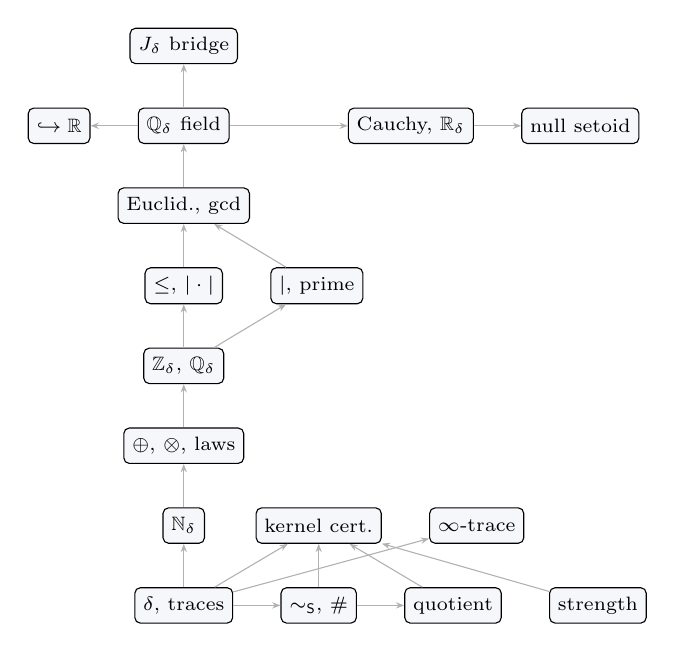
\begin{tikzpicture}[
  node distance=0.55cm and 0.4cm,
  every node/.style={font=\scriptsize, draw, rounded corners=2pt,
    minimum height=0.45cm, inner sep=3pt, fill=codebg},
  arr/.style={-{Stealth[length=3pt]}, thin, gray!60}
]
\node (basic) {$\delta$, traces};
\node[right=0.6cm of basic] (sd) {$\sim_{\mathsf{S}}$, $\mathbin{\#}$};
\node[right=0.6cm of sd] (quot) {quotient};
\node[right=0.6cm of quot] (str) {strength};
\node[above=of basic] (orbit) {$\mathbb{N}_\delta$};
\node[above=of sd] (kernel) {kernel cert.};
\node[above=of orbit] (oa) {$\oplus$, $\otimes$, laws};
\node[above=of oa] (ir) {$\mathbb{Z}_\delta$, $\mathbb{Q}_\delta$};
\node[above=of ir] (io) {$\leq$, $|\cdot|$};
\node[right=0.6cm of io] (od) {$\mid$, prime};
\node[above=of io] (oe) {Euclid., gcd};
\node[above=of oe] (rf) {$\mathbb{Q}_\delta$ field};
\node[right=1.5cm of rf] (rc) {Cauchy, $\mathbb{R}_\delta$};
\node[right=0.6cm of rc] (rns) {null setoid};
\node[left=0.6cm of rf] (rcomp) {$\hookrightarrow \mathbb{R}$};
\node[above=of rf] (jcost) {$J_\delta$ bridge};
\node[right=0.6cm of kernel] (tc) {$\infty$-trace};

\draw[arr] (basic) -- (orbit);
\draw[arr] (basic) -- (sd);
\draw[arr] (sd) -- (quot);
\draw[arr] (basic) -- (kernel);
\draw[arr] (sd) -- (kernel);
\draw[arr] (quot) -- (kernel);
\draw[arr] (str) -- (kernel);
\draw[arr] (orbit) -- (oa);
\draw[arr] (oa) -- (ir);
\draw[arr] (ir) -- (io);
\draw[arr] (ir) -- (od);
\draw[arr] (io) -- (oe);
\draw[arr] (od) -- (oe);
\draw[arr] (oe) -- (rf);
\draw[arr] (rf) -- (rc);
\draw[arr] (rc) -- (rns);
\draw[arr] (rf) -- (rcomp);
\draw[arr] (rf) -- (jcost);
\draw[arr] (basic) -- (tc);
\end{tikzpicture}
\caption{Construction dependency graph. Lower constructions feed higher ones.
The graph is the arithmetic and real-completion spine. The current formal
dependency extends this spine with trace logic, formal-system embedding,
admissible-foundation inevitability, recognizer cost bridge, native-cost
blocker ledger, and the conditional universal-foundation certificate.}
\label{fig:deps}
\end{figure}

\subsection{Strength audit summary}

Table~\ref{tab:audit} records the strength tag and key result for each
construction layer.

\begin{table}[ht]
\centering\small
\begin{tabular}{lll}
\toprule
\textbf{Construction} & \textbf{Strength} & \textbf{Key result} \\
\midrule
Traces, concatenation    & $\delta$-only & Associativity of $\mathbin{\|}$ \\
$\sim_{\mathsf{S}}$, $\mathbin{\#}$, substitution
                         & $\delta$-only & Reflexivity, consistency \\
Quotient recursion       & $\delta$-only & Well-defined descent \\
$\mathbb{N}_\delta$      & $\delta$-only & Successor injectivity \\
Strength tags            & $\delta$-only & (definitional) \\
Kernel certificate       & $\delta$-only & Thm.~\ref{thm:kernel} \\
$\oplus$, $\otimes$, laws & $\delta$-only & Thm.~\ref{thm:orbit}: display faithfulness \\
$\mathbb{Z}_\delta \cong \mathbb{Z}$
                         & $\delta$-only & Thm.~\ref{thm:int}: ring isomorphism \\
Order, absolute value    & $\delta$-only & Thm.~\ref{thm:permission}(a)--(b) \\
Divisibility, primality  & $\delta$-only & Thm.~\ref{thm:permission}(c)--(d) \\
Euclidean div., gcd      & $\delta$-only & Thm.~\ref{thm:permission}(e)--(f) \\
$\mathbb{Q}_\delta$ field & $\delta$-only & Thm.~\ref{thm:rat}: field isom. \\
Infinite trace boundary  & $\delta$ + trace-cl. & Cauchy boundary \\
Cauchy completion        & $\delta$ + trace-cl. & $\mathbb{R}_\delta$ quotient \\
Classical embedding      & classical ext. & $\iota : \mathbb{Q}_\delta
  \hookrightarrow \mathbb{R}$ \\
Null-distance setoid     & $\delta$ + trace-cl. & Conditional certificate \\
$J_\delta$ bridge        & $\delta$-only (bridge) & Thm.~\ref{thm:bridge} \\
Trace logic              & $\delta$-only & Stable predicates and connectives \\
Formal-system embedding  & $\delta$-only & Expressive systems admit PRC embeddings \\
Admissible inevitability & $\delta$-only & Parsed foundations contain PRC core \\
Recognizer cost bridge   & classical ext. & Thm.~\ref{thm:recognizer-cost} \\
Cost joint (resolved)    & mixed & Form forced; unit a gauge (Sec.~\ref{sec:native-cost-blocker}) \\
Universal conditional cert. & mixed & Built conditional certificate \\
\bottomrule
\end{tabular}
\caption{Strength audit. The finite arithmetic, trace-logic, formal-system,
and inevitability layers are $\delta$-only. The internal
real-completion layer uses trace-closure. The recognizer bridge to the
continuous Law-of-Logic theorem and the raw classical embedding boundary use
classical extension. All listed certificates have no unfinished proof
obligations. The cost-forcing joint is resolved: $\delta$ forces the cost form
and a unit calibration fixes the gauge that selects $J$
(Section~\ref{sec:native-cost-blocker}).}
\label{tab:audit}
\end{table}

%% ===================================================================
\begin{thebibliography}{99}

\bibitem{Aczel1966}
J.~Acz\'el,
\emph{Lectures on Functional Equations and Their Applications},
Academic Press, 1966.

\bibitem{Conway1976}
J.~H.~Conway,
\emph{On Numbers and Games},
Academic Press, 1976.

\bibitem{Lawvere1964}
F.~W.~Lawvere,
``An Elementary Theory of the Category of Sets,''
\emph{Proc.\ Natl.\ Acad.\ Sci.\ USA}, 1964.

\bibitem{MartinLof1984}
P.~Martin-L\"of,
\emph{Intuitionistic Type Theory},
Bibliopolis, 1984.

\bibitem{HoTT2013}
The Univalent Foundations Program,
\emph{Homotopy Type Theory: Univalent Foundations of Mathematics},
Institute for Advanced Study, 2013.

\bibitem{Baez2006}
J.~C.~Baez,
``Quantum Quandaries: A Category-Theoretic Perspective,''
in \emph{The Structural Foundations of Quantum Gravity},
Oxford University Press, 2006.

\bibitem{SpencerBrown1969}
G.~Spencer-Brown,
\emph{Laws of Form},
George Allen and Unwin, 1969.

\bibitem{Washburn2026LogicFE}
J.~Washburn,
``A Functional-Equation Encoding of Logical Consistency on Continuous
Positive-Ratio Comparisons: A Conditional Rigidity Theorem,''
draft, 2026.

\bibitem{Washburn2026Arithmetic}
J.~Washburn,
``Arithmetic from the Law of Logic: The Continuous Positive-Ratio
Realization,''
draft, 2026.

\bibitem{Washburn2026Geometry}
J.~Washburn,
``The Unified Forcing Chain: From Recognition Geometry to the Law of
Logic,''
draft, 2026.

\bibitem{WashburnZlatanovic2026}
J.~Washburn and Z.~Zlatanovi\'c,
``Uniqueness of the Canonical Reciprocal Cost,''
\emph{Axioms}, 2026.

\bibitem{Lean4}
The Lean~4 Theorem Prover and Mathlib Community,
Lean~4 and Mathlib documentation and library sources, 2026.

\end{thebibliography}

\end{document}
